\documentclass{article}

\usepackage{amsmath}
\usepackage{amssymb}
\usepackage{listings}

\usepackage[utf8]{inputenc}
 
\usepackage{listings}
\usepackage{color}

\usepackage{graphicx}
\graphicspath{ {./} }

\usepackage[T1]{fontenc}
\usepackage{libertine}
\usepackage[scaled=0.85]{beramono}

\lstset{
  basicstyle=\ttfamily\small,
  breakatwhitespace=false,     
  breaklines=true,         
  captionpos=b,          
  keepspaces=true,         
  showspaces=false,        
  showstringspaces=false,
  showtabs=false,          
  tabsize=2
}
 
\lstdefinelanguage{logic}{
  morekeywords={
    datatype,
    type,
    fun,
    predicate,
    only, if, then, else,
    and, or, not,
    lemma,
    theorem,
    of
  }
}
 


\title{Formal Theory of Concurrent ML}
\author{Thomas Logan}
\begin{document}

\maketitle
\pagenumbering{gobble}

\newpage
\pagenumbering{arabic}


\section{Abstract}
For this master's thesis, I have developed a formal framework for analysis of
a concurrent language, along with an initial formal analysis.  The language under analysis is
a very simplied version of \textit{Concurrent ML} \cite{concurrent_ml}. The formal analysis
is a recast of an informal analysis developed by Xiao and Reppy \cite{specialization}. It
categorizes communication described by the language into simple topologies. One description of
topologigies is static; that is, it describes topologies in terms of the finite structure of
programs.  Another description is dynamic; that is, it describes topologies in terms of running
a program for an arbitrary number of steps. The main formal theorem states that the static
analysis is sound with respect to the dynamic analysis. Two versions of the static analysis
have been developed so far, one with lower precision, and one with higher precision. The higher
precision analysis is closer to the work by Reppy and Xiao, but has greater complexity than the
lower precision analysis. The proofs for the soundness theorem of the lower precision analysis
have been mechannically verified using Isabelle \cite{isabelle}, while the higher precision
analysis is currently under development. Indeed, one of the motivations for placing the theory
in a formal setting is to enable gradual extension of analysis and language without introducing
uncaught bugs in the definitions or proofs. The definitions used in this formal theory differ
significantly from that of Reppy and Xiao, in order to aid formal reasoning. Although the
definitions are structurally quite different, their philsophocial equivalence is hopefully
apparent. Thus, recasting Reppy and Xiao's work was far more nuanced than a straight forward
syntactic transliteration. In this formal theory, the dynamic semantics of Concurrent ML is
defined by a small-step operational semantics. The static semantics is an instance of 0CFA
\cite{0cfa}, defined in terms of nonequational constraints \cite{program_analysis}.

\section{Introduction}
In programming languages, concurreny is a program structuring technique that allows evaluation
steps to hop back and forth between disjoint syntactc structures within a program. It is useful
when conceptually distinct tasks need to overlap in time, but are easier to understand if they
are written as distinct structrues within the program. Concurrent languages may also allow the
evaluation order between steps of expressions to be nondeterministic. If it's not necessary for
tasks to be ordered in a precise way, then it may be better to allow a static or dynamic
scheduler pick the most efficient execution order. A common use case for concurrent languages
is for programs that interact with humans, in which a program has to process various requests
while remaining responsive to subsequent user inputs, and it must continually provide the user
feedback with latest information it has processed.

\textit{Concurrent ML} is a particularly elengant concurrent programming language.
It features threads, which are pieces of code allowed to have a wide range of
evaluation orders relative to code encapsulated in other threads. Its synchronization
mechanism can mandate the execution order between parts of separate threads. It is often the
case that synchronization is necessary when data is shared. Thus, in \textit{Concurrent ML},
synchronization is inherent in communication. Threads are spawned asynchronously; that is, the
parent thread need not wait for the spawned thread to terminate before it resumes evaluation.
Indeed, if that were the case, then threads would be useless. Additional threads can be spawned
in order to share data asynchronously, which can provide better usability or performance under
some circumstances.

Threads communicate by having shared access to a common channel.  A channel can be used to
either send data or receive data.  When a thread sends on a channel, another thread must
receive on the same channel before the sending thread can continue.  Likewise, when a thread
receives on a channel, another thread must send on the same channel before the receiving thread
can continue.

\begin{lstlisting}[language=ML, escapechar=\%]
  type thread_id
  val spawn : (unit -> unit) -> thread_id

  type 'a chan
  val channel : unit -> 'a chan
  val recv : 'a chan -> 'a
  val send : ('a chan * 'a) -> unit
  \end{lstlisting}

A given channel can have any arbitrary number of threads sending or receiving data on it over
the course of the program's execution. A simple example, derived from Reppy's book
\textit{Concurrent Programming in ML} \cite{concurrent_ml}, illustrates these essential
features.

The implementation of \lstinline{Serv} defines a server that holds a number in its state.
When a client gives the server a number \lstinline{v}, the server gives back the number in
its state, and updates its state with the number \lstinline{v}.  The next client request will
get the number \lstinline{v}, and so on. Essentially, a request and reply is equivalent
to reading and writing a mutable cell in isolation. The function \lstinline{make} makes a new
server, by creating a new channel \lstinline{reqCh}, and a loop \lstinline{loop} which listens
for requests. The loop expects the request to be composed of a number \lstinline{v} and a
channel \lstinline{replCh}. It sends its current state's number on \lstinline{replCh} and
update's the loop's state with the request's number \lstinline{v}, by calling the loop with a
new that number. The server is created with a new thread with the initial state \lstinline{0}
by calling \lstinline[language=ML]{spawn (fn () => loop 0)}. The request channel is returned
as the handle to the server.  The function \lstinline{call} makes a request to the passed in
server server \lstinline{server} with a number \lstinline{v} and returns a number from the
server. Internally, it extracts the request channel \lstinline{reqCh} from the
server handle and creates a new channel \lstinline{replCh}. It makes a request to the server
with the number \lstinline{v} and the reply channel \lstinline{replCh} by calling
\lstinline{send (reqCh, (v, replCh))}. Then it receives the reply with the new number by
calling \lstinline{recv replCh}.


\begin{lstlisting}[language=ML, escapechar=\%]
  signature SERV = sig 
    type serv
    val make : unit -> serv
    val call : serv * int -> int
    end

  structure Serv : SERV = struct 

    datatype serv = S of (int * int chan) channel 

    fun make () = let 
      val reqChn = channel ()
      fun loop state = let
        val (v, replCh) = recv reqChn in 
        send (replCh, state);
        loop v end in
      spawn (fn () => loop 0);
      S reqChn end 

    fun call (server, v) = let 
      val S reqChn = server
      val replChn = channel () in 
      send (reqCh, (v, replCh));
      recv replChn end

    end
  \end{lstlisting}


\textit{Concurrent ML} actually allows for events other than sending and receiving to
occur during synchronization. In fact, the syncronization mechanism is decoupled from
events, like sending and receiving, much in the same way that function application is decoupled
from function abstraction. Sending and receiving events are represented by \lstinline{sendEvt}
and \lstinline{recvEvt} and synchronization is represented by \lstinline{sync}.

\begin{lstlisting}[language=ML, escapechar=\%]
  type 'a event
  val sync : 'a event -> 'a

  val recvEvt : 'a channel -> 'a event
  val sendEvt : 'a channel * 'a -> unit event

  fun send (ch, v) = sync (sendEvt (ch, v))
  fun recv v = sync (recvEvt v)
  \end{lstlisting}

An advantageous consequence of decoupling syncronization from events, is that events can be
combined with other events via event combinators, and synchronized on exactly once. One such
event combinator is \lstinline{choose}, which constructs a new event consisting of two
constiuent events, such that when sycnronized on, exactly one of the two events may take
effect. There are many other useful combinators, such as the \lstinline{wrap} and
\lstinline{guard} combinators designed by Reppy[8]. Additionally, Donnelly and Fluet extended
\textit{Concurrent ML} with the \lstinline{thenEvt} combinator described in their work on
transactional events \cite{transactional_events}. Transactional events enable more robust
structuring of programs by allowing non-isolated code to be turned into isolated code via
the \lstinline{thenEvt} combinator, rather than duplicating code with the addition of stronger
isolation. When the event constructed by the \lstinline{thenEvt} combinator is is synchronized
on, either all of its constituent events and abstractions evaluate in isolation, or none
evaluates.

\begin{lstlisting}[language=ML, escapechar=\%]
  val choose : 'a event * 'a event -> 'a event
  val thenEvt : 'a event * ('a -> 'b event) -> 'b event
  \end{lstlisting}

\section{Syncrhonization Implementation}
The implementation of synchronization requires determining which threads should 
synchronization, and which threads should be dispatched. The more amount of information needed
to determine this scheduling, the higher the performance penality. A uniprocessor
implementation of synchronization can have very little penalty. Since only one thread can make
progress at a time, only one thread requests synchronization at a time, meaning the scheduler
won't waste steps checking for threads competing for the same synchronization opportunity,
before dispatching. A multiprocessor implementation, on the other hand, must consider that
competing threads may exists, therefore peform additional checks. Addtionally, there may be 
overhead in sharing data between processors due to memory hiearchy designs \cite{}. 

One way to lower synchronization and communication costs is to use specialized implementations
for channels that have no more than one thread ever sending or receiving on them.  These
specialized implementations would avoid unnecessary checks for competing threads.
Concurrent ML does not feature multiple kinds of channels distinguished by their communication
topologies, i.e. the number of threads that may end up sending or receiving on the channels.
However, channels can be classified into various topologies simply by counting the number of
threads per channel during the execution of a program.  A many-to-many channel has any number
of sending threads and receiving threads; a one-to-many channel has one or no sending thread and
any number of receiving threads; a many-to-one channel has any number of sending threads and one or
no receiving threads; a one-to-one channel has one or none of each; a one-shot channel has
exactly one sending attempt.

The implementation of \lstinline{Serv} is annoted to indicate the communication topologies
derived from its usage. Since there are four threads that make calls to the server, the
server's particular \lstinline{reqCh} has four senders.  Servers are created with only one
thread listening for requests, so the \lstinline{reqCh} of this server has just one receiver.
So the server's \lstinline{reqCh} is classified as many-to-one. Each use of call creates a distinct
new channel \lstinline{replCh} for receiving data.  The function call receives on the channel
once and the server sends on the channel once, so each instance of \lstinline{replCh} is
one-shot.

\begin{lstlisting}[language=ML, escapechar=\%]
  val server = Serv.make ()
  val _ = spawn (fn () => Serv.call (server, 35))
  val _ = spawn (fn () => 
    Serv.call (server, 12); 
    Serv.call (server, 13))
  val _ = spawn (fn () => Serv.call (server, 81))
  val _ = spawn (fn () => Serv.call (server, 44))
  \end{lstlisting}

\begin{lstlisting}[language=ML, escapechar=\%]
  structure Serv : SERV = struct 

    datatype serv = S of (int * int chan) channel 

    fun make () = let 
      val reqChn = FanIn.channel ()
      fun loop state = let
        val (v, replCh) = FanIn.recv reqChn in 
        OneShot.send (replCh, state);
        loop v end in
      spawn (fn () => loop 0);
      S reqChn end 

    fun call (server, v) = let 
      val S reqChn = server
      val replChn = OneShot.channel () in 
      FanIn.send (reqCh, (v, replCh));
      OneShot.recv replChn end

    end
  \end{lstlisting}

The right implementation choice can be determined by counting the number threads used during
the execution of a program. However, some programs run forever, so it may never be possible to
count all the threads. Instead, by using a static analysis it's possible to determine an
estimate from the finite structure of programs. A static analysis that describes communication
topologies of channels has practical benefits in at least two ways.  It can highlight which
channels are candidates for optimized implementations of communication; or in a language
extension allowing the specification of specialized channels, it can conservatively verify
their correct usage. Without a static analysis to check the usage of the special channels, one
could inadvertently use a one-shot channel for a channel that has multiple senders, thus
violating the intended semantics. 

The utility of the static analysis additionally depends on it being precise, sound, and
computable. The analysis is precise iff there exist programs about which the analysis
describes information that is not directly observable. The analysis is sound iff the
information it describes about a program is the same or less precise than the dynamic
semantics of the program. The analysis is computable iff there exists an algorithm that
determines all the values described by the analysis on any input program.

There are a large number of static analyses with a variety of practical uses. The most familiar
kind of static analyses are type systems.  A type system statically evaluates expressions
in programs to abstract categories known as types. In a sound type system, if an expression is
well typed, then it can be dynamically evaluated (without error). Some expressions cannot be
typed, indicating the possiblity that the expression cannot be dynamically evaluated. Type
systems can improve debugging by pointing out errors that may be infrequently executed. They
can also improve execution speeds of safe languages by rendering dynamic checks unnecessary.  

Other kinds of analysis are useful for describing opportunities for program optimizations.
A data flow analysis describes how data flows from one point to another in the program.
A data flow analysis for available expressions tracks the expressions have already been
computed by every program point. Using this information, redundant code can be detected and
removed to improve performance.

In the following example, an analysis for available expressions would track
\lstinline{(!x + 1)} and \lstinline{(w - 3)} to remain available from line 5 all the way until
the end of the program, meaning those two redudandt expressions in line 8 can be swapped with
the results of their evaluation. In contrast, \lstinline{(!y + 2)} would be tracked as avaiable
from line 5 until line 7. It would be unavailable after line 7 because the number in
\lstinline{y} is modifided in line 7, changing the how the expression would evaluate after
that.

\begin{lstlisting}[language=ML, escapechar=\%]
  1. let
  2.   val w = 4
  3.   val x = ref 1
  4.   val y = ref 2
  5.   val z = (!x + 1) + (!y + 2) + (w - 3)
  6.   val w = 1 in
  7.   y := 0;
  8.   (!y + 2) - (!x + 1) * (w - 3) end
  \end{lstlisting}



A dataflow analysis for liveness tracks the set of stored valued that are used in the
remainder of the program. Using this information, unused code can
be detected and removed to improve performance. There are other uses of this analysis, as well.
In this work, the liveness of channels is tracked to distinguish between distinct channels with
the same name. 

In the following example, an analysis for liveness of values stored in names and references
would track \lstinline{x} to be live from line 7 until line 5. Above line 5 there are no uses
of \lstinline{x}, so it would not be live. Since the name \lstinline{x} at line 2 is not used,
line 2 can be removed. The reference contained in \lstinline{z} would be
live from line 7 until line 6, where it is assigned. There is no deference of lstinline{z}
above line 6, so it not live from there until the beginning. Since the reference contained in
\lstinline{z} is not live at line 4, line 4 can be removed.

\begin{lstlisting}[language=ML, escapechar=\%]
  1. let 
  2.   val x = 1  
  3.   val y = 2
  4.   val z = ref (4 * 73)
  5.   val x = 4 in 
  6.   z := 1; 
  7.   x * !z end
  \end{lstlisting}

The information at each program point is derived from control structures in the program, which
dictate how information flows between program points. Some uses of control structures are
literally represented in the syntax, such as the sequencing of namings and assignments in the
previous examples. Other uses of control structures may be indirectly represented through
names. Function application is a control structure that allows a calling piece of code to
flow into a function abstraction's code.  Function abstractions can be named, which allows
multiple pieces of code to all flow into into the same section of code. The name adds an
additional step in to uncover control structures, and determine data flow.
Additionally, in languages with higher order functions and recursion, such as those in the Lisp
and ML families, it may be impossible to determine all the function abstractions that
expressions resolve to. However, a control flow analysis can reveal a good
approximation of the control structures and values that have been obfuscated by higher order
function abstractions.  Uncovering the the control structures depends on resolving expressions
to values, and resolving expressions to values depends on on unconvering the control
structures. The mutual dependency means that control flow analysis is a form of
static semantics that describes approximate evaluations of programs. In this work, control flow
analysis for tracking certain kinds of values, like channels and events, in addition to
constructing precise data flow analysis. 

--------

Analyses can be described in a variety of ways.  An algorithm that take programs as input and
produce behavior information as output are necessary for automation in compilers.  A
specification that states a proposition in terms of programs and execution information may be
more suitable for showing clarity of meaning and correctness with respect to the operational
semantics.  The specification can be translated into an algorithm involving two parts.  The
first part generates a comprehensive set of data structures representing constraints of all
program points, mirroring the specification's description, and the second part solves the
constraints.

For a subset of Concurrent ML without event combinators, Reppy and  Xiao developed an
efficient algorithmic analysis that determines for each channel all abstract threads that send
and receive on it.  The algorithm depends on each primitive operation in the program being
labeled with a program point.  A sequence of program points ordered in a valid execution
sequence forms a control path.  Distinction between threads in a program can be inferred from
whether or not their control paths diverge.  

The algorithm proceeds in multiple steps that produce intermediate data structures, used for
efficient lookup in the subsequent steps.  It starts with a control-flow analysis[12, 13] that
results in multiple mappings. One mapping is from variables to abstract values that may bind to
the variables.  Another mapping is from channel-bound variables to abstract values that are
sent on the respective channels.  Another is from function-bound variables to abstract values
that are the result of respective function applications.  It constructs a control-flow graph 
with possible paths for pattern matching and thread spawning determined directly from the
primitives used in the program.  Relying on information from the mappings to abstract values,
it constructs the possible paths of execution via function application and channel
communication.  It uses the graph for live variable analysis of channels, which limits the
scope for the remaining analysis.  Using the spawn and application edges of the control-flow
graph, the algorithm then performs a data-flow analysis to determine a mapping from program
points to all possible control paths leading into the respective program points.  Using the
CFA's mappings to abstract values, the algorithm determines the program points for sends and
receives per channel variable.  Then it uses the mapping to control paths to determine all
control paths that send or receive on each channel, from which it classifies channels as
one-shot, one-to-one, many-to-one, one-to-many, or many-to-many.

Reppy and Xiao informally prove soundness of their analysis by showing that their analysis
claims that more than one thread sends (or receives) on a channel if the execution allows more
than one to send (or receive) on a that channel.  The proof of soundness depends on the
ability to relate the execution of a program to the static analysis of a program.  The static
analysis describes threads in terms of control paths, since it can only describe threads in
terms of statically available information. Thus, in order to describe the relationship between
the threads of the static analysis and the operational semantics, the operational semantics is
defined as stepping between sets of control paths paired with terms.  Divergent control paths
are added whenever a new thread is spawned.

The syntax, semantics, and analysis need to describe many details.  Proving propositions
relating all of these definitions requires manipulation of all those details.  To ensure the
correctness of proofs, it is necessary to check that there are no subtle errors in the
definitions or proofs.  Proofs in general require many subtle manipulations of symbols.  The
difference between a false statement and a true statement can often be difficult to spot, since
the two may be very similar lexically.  However, a mechanical proof checker, such as the one in
Isabelle, has no difficulty discerning between valid and invalid derivations of statements.
Mechanical checking of proofs can notify us of errors in the proofs or definitions far better
and faster than manual checking.  I have already benefitted from Isabelle's proof checker in
order to correctly define the language semantics and abstract value flow analysis for this
work.  While trying to prove soundness of the analysis, the proof assistant would not accept my
proof unless I provided derivation of facts that I believed to be false.  I determined that my
intuition was correct but my definitions had errors.  After correcting the errors, I was able
to complete the proof, such that the proof checker was satisfied.


\section{Hypothesis}
I will derive a static analysis from Reppy and Xiao's algorithm, describing for each channel in
a program, all threads that possibly send or receive on the channel.  Additionally, it will
classify channels as one-shot, one-to-one, one-to-many, many-to-one, or many-to-many.  Instead of
Serrano's algorithm[18] for the CFA used in Reppy and Xiao's algorithm, I will define a
constraint-based specification and algorithm for the CFA.  The method of determining topologies
will be fairly similar to Reppy and Xiao's.  The analysis of this work will also consider event
combinators, which are not considered in Reppy and Xiao's work.  I will show that the static
analysis is informative by demonstrating programs for which the static analysis classifies some
channels as many-to-one, one-to-many, and so on.  I will show that the static analysis is sound by
showing that for any program, the execution of the program results in the same sends and
receives or fewer compared to the possible sends and receives described by the analysis.  I
will show that the static analysis is computable by demonstrating the existence of a
computable function that takes any program as input and generates all sends and receives
described by the analysis.


\section{Evaluation}
The main contributions of this work will be formal and mechanically verified proofs of
communication properties of Concurrent ML, including an analysis derived from Reppy and Xiao's
analysis.  This work extends that of Reppy and Xiao by demonstrating formal proofs of soundness
and extending the analysis to encompass event combinators for choice and transactions.


\section{Architecture}
To enable mechanical verification of the correctness of the proofs, I will construct the
semantics, analysis and theorems in the formal language of Isabelle/HOL.  To aid the
development of formal proofs, I will design the analysis as a declarative specification as
opposed to an algorithm.  However, the declarative analysis will make the proof of
computability less direct.  To aid the scrutiny of the theorems' adequacy, I will express the
definitions and propositions with the fewest number of structures, judgements, inferences rules
, and axioms necessary. In order to relate the analysis to the operational semantics, I will
borrow Reppy and Xiao's strategy of stepping between sets of control paths tied to terms.

In this thesis work, I'm interested in communication topology soundness, rather than flow
soundness.  Nevertheless, I will need to prove additional flow soundness theorems en route to
proving communication topology soundness.  Restricting the grammar to a form that requires
every abstraction and application to be bound to a variable would allow the operational
semantics to maintain static term information necessary for proofs of flow soundness[3, 5].
The semantics would be defined as an environment based operational semantics, rather than a
substitution based operational semantics.  By avoiding simplification of terms in the
operational semantics, it will be possible to relate the abstract values of the analysis to the
values produced by the operational semantics, which in turn is relied on to prove flow
soundness.


I will incorporate the restricted grammar and the environment based semantics into this work.
The restricted grammar is impractical for a programmer to write, yet it is still practical for
a language under automated analysis since there is a straight forward procedure to transform
more flexible grammars into the restricted form as demonstrated by Flanagan et al [2].
Additionally, the restricted grammar melds nicely with the control path semantics.  Instead of
defining additional meta-syntax for program points of primitive operations, I can simply use
the required variables of the restricted grammar to identify program points, and control paths
will simply be sequences of let bound variables. A modification of Listing 2 illustrates the
restrictive grammar applied to Concurrent ML.


\section{Implementation}
We describe possible implementations of specialized and unspecialized Concurrent ML using
feasible low-level thread-centric features such as wait and poll.  The thread-centric approach
allows us to focus on optimizations common to many implementations by decoupling the
implementation of communication features from thread scheduling and management.  Depending on
the low level features provided by existing language implementations, Concurrent ML could be
implemented in terms of lower level features, as is the case in SML/NJ and MLton.  It could
also be implemented as primitive features within a compiler and runtime or interpreter.
Analyzing and optimizing Concurrent ML would require treating the language as an object, so
implementing its features as primitives would make the most sense.  Thus, one can think of the
implementation shown here as an intermediate representation presented with concrete syntax.

\begin{lstlisting}[language=ML, escapechar=\%]
  signature CHANNEL = sig
    type 'a channel 
    val channel : unit -> 'a chan
    val send : 'a channel * 'a -> unit
    val recv : 'a channel -> 'a
    end     
\end{lstlisting}


The benefits of specialization would be much more significant in multiprocessor
implementations rather than single processor implementations.  A single processor
implementation could avoid overhead caused by contention to acquire locks, by coupling the
implementation of channels with scheduling and only scheduling send and recv operations when no
other pending operations have yet to start or have already finished.  Reppy's implementation of
Concurrent ML uses SML/NJ's first class continuations to implement scheduling and communication
as one with low overhead.  However, a multiprocessor implementation would allow threads to run
on different processors for increased parallelism and would not be able to mandate when threads
are attempted relative to others without losing the parallel advantage.  The cost of trying to
achieve parallelism is increased overhead due to contention over acquiring locks.

A channel can be in one of three states.  Either some threads are trying to send through it,
some threads are trying to receive from it, or no threads are trying to send or receive.
Additionally a channel is composed of a mutex lock, so that send and recv operations can yield
to each other when updating the channel state.  When multiple threads are trying to send on a
channel, the channel is associated with a queue consisting of messages to be sent, along with
conditions waited on by sending threads. When multiple threads are trying to receive on a
channel, the channel is associated with a queue consisting of initially empty cells accessible
by receiving threads and conditions waited on by the receiving threads. The three states are
represented by the datatype chan\_content.  The channel is represented by the channel datatype,
which is composed of a reference to chan\_content and a mutex lock.  

The send operation acquires the channel's lock to ensure that it updates the channel based on
any one of its latest state.  If there are threads trying to receive from the channel, the send
operation dequeues an item from the state's associated queue.  The item consists of a condition
waited on by a receiving thread and an empty cell that can be accessed by the receiving thread.
It deposits the message in the cell and signals on the condition, updates the channel state to
inactive if there are no further receiving threads waiting, then releases the lock, signals on
the condition and returns the unit value.  If there are no threads trying to receive from the
channel, the send operation updates the channel state to that of trying to send with an
additional condition and message in the associated queue.  It releases the lock and waits on
the enqueued condition.  Once a receiving thread signals on the same condition, the send
operation returns with the unit value.

The recv operation acquires the channel's lock to ensure that it updates the channel based on
any one of its latest state.  If there are threads trying to send on the channel, the recv
operation dequeues an item from the state's associated queue.  The item consists of a condition
waited on by a sending thread along with a message to be sent.  It signals the condition and
updates the channel state to inactive if there are no further sending threads waiting, then
releases the lock and returns the sent message.  If there are no threads trying to send on the
channel, the recv operation updates the channel state to that of trying to receive with an
additional condition and empty cell in the associated queue.  It releases the lock and waits on
the enqueued condition.  Once a sending thread signals on the same condition, the recv
operation returns with the value deposited in the cell by a sending thread.

\begin{lstlisting}[language=ML, escapechar=\%]

  structure ManyToManyChan : CHANNEL = struct
    type message_queue = 'a option ref queue

    datatype 'a chan_content = 
      Send of (condition * 'a) queue | 
      Recv of (condition * 'a option ref) queue | 
      Inac

    datatype 'a channel =
      Chn of 'a chan_content ref * mutex_lock 

    fun channel () = Chn (ref Inac, mutexLock ())

    fun send (Chn (conRef, lock)) m = 
      acquire lock;
      (case !conRef of
        Recv q => let
          val (recvCond, mopRef) = dequeue q in
          mopRef := Some m;
          if (isEmpty q) then conRef := Inac else (); 
          release lock; signal recvCond; () end |
        Send q => let
          val sendCond = condition () in
          enqueue (q, (sendCond, m));
          release lock; wait sendCond; () end |
        Inac => let
          val sendCond = condition () in
          conRef := Send (queue [(sendCond, m)]);
          release lock; wait sendCond; () end)

    fun recv (Chn (conRef, lock)) =  
      acquire lock;
      (case !conRef of 
        Send q => let
          val (sendCond, m) = dequeue q in
          if (isEmpty q) then
            conRef := Inac
          else
            (); 
          release lock; signal sendCond; m end |
        Recv q => let
          val recvCond = condition ()
          val mopRef = ref None in
          enqueue (q, (recvCond, mopRef));
          release lock; wait recvCond;
          valOf (!mopRef) end |
        Inac => let
          val recvCond = condition ()
          val mopRef = ref None in
          conRef := Recv (queue [(recvCond, mopRef)]);
          release lock; wait recvCond;
          valOf (!mopRef) end)

    end

  \end{lstlisting}


Implementation of one-to-many channels, compared to that of many-to-many channels, requires fewer
steps to synchronize and can execute more steps outside of critical regions, which reduces
contention for locks.  A channel is composed of a lock and one of three possible states, as is
the case for many-to-many channels.  However, the state of a thread trying to send need only be
associated with one condition and one message.  

The send operation checks if the channel's state is inactive and tries to use the
compareAndSwap operator to transactionally update the state of the channel to that of trying to
send.  If successful, it simply waits on sendCond, the condition that a receiving thread will
signal on, and then returns the unit value.  If the transactional update fails and the state is
that of threads trying to receive on the channel, then the send operation acquires the lock,
then dequeues an item from the associated queue where the item consists of recvCond, a
condition waited on by a receiving thread, and a cell for depositing the message to that
receiving thread.  It deposits the message in the cell, updates the state to inactive there are
no further items on the queue, then releases the lock.  Then it signals on the condition and
returns the unit value. The lock is acquired after the state is determined to be that of
threads trying to receive, since the expectation is that the current thread is the only one
that tries to update the channel from that state.  If the communication topology analysis were
incorrect and and there were actually multiple threads that could call the send operation, then
there might be data races.  Likewise, due to the expectation of a single thread sending on the
channel, the send operation should never witness the state of threads already trying to send.

The recv operation acquires the lock and checks the state of the channel, just as the recv
operation for many-to-many channels.  If the channel is in a state where there is no already
trying to send, then it behaves the same as the recv operation of many-to-many channels. If
there is already a thread trying to receive, then it updates the state to inactive and releases
the lock.  Then it signals on the state's associated condition, which is waited on by a sending
thread, and returns the states' associated message.

  \begin{lstlisting}[language=ML, escapechar=\%]

    structure FanOutChan : CHANNEL = struct

    datatype 'a chan_content =
      Send of condition * 'a |
      Recv of (condition * 'a option ref) queue  |
      Inac

    datatype 'a channel =
      Chn of 'a chan_content ref * mutex_lock

    fun channel () = Chn (ref Inac, mutexLock ())

    fun send (Chn (conRef, lock)) m = let
      val sendCond = condition () in
      case cas (conRef, Inac, Send (sendCond, m)) of
        Inac => (* conRef already set *)
          wait sendCond; () |
        Recv q => 
        (* the current thread is
          * the only one that updates from this state *)
          acquire lock;
          (let
            val (recvCond, mopRef) = dequeue q in
            mopRef := Some m; 
            if (isEmpty q) then conRef := Inac else (); 
            release lock; signal (recvCond);
            () end) |
        Send _ => raise NeverHappens end

    fun recv (Chn (conRef, lock)) =
      acquire lock;
      (case !conRef of
        Inac => let
          val recvCond = condition ()
          val mopRef = ref None in
          conRef := Recv (queue [(recvCond, mopRef)]);
          release lock; wait recvCond;
          valOf (!mopRef) end |
        Recv q => let
          val recvCond = condition () 
          val mopRef = ref None in
          enqueue (q, (recvCond, mopRef));
          release lock; wait recvCond;
          valOf (!mopRef) end |
        Send (sendCond, m) =>
          conRef := Inac;
          release lock;
          signal sendCond;
          m end) 

    end 
  \end{lstlisting}

The implementation of many-to-one channels is very similar to that of one-to-many channels.

\begin{lstlisting}[language=ML, escapechar=\%]
  structure FanInChan : CHANNEL = struct

  datatype 'a chan_content =
    Send of (condition * 'a) queue |
    Recv of condition * 'a option ref |
    Inac

  datatype 'a channel =
    Chn of 'a chan_content ref * mutex_lock

  fun channel () = Chn (ref Inac, mutexLock ())

  fun send (Chn (conRef, lock)) m = 
    acquire lock;
    case !conRef of
    Recv (recvCond, mopRef) => 
      mopRef := Some m; conRef := Inac;
      release lock; signal recvCond;
      () |
    Send q => let
      val sendCond = condition () in
      enqueue (q, (sendCond, m));
      release lock; wait sendCond;
      () end |
    Inac => let
      val sendCond = condition () in
      conRef := Send (queue [(sendCond, m)])
      release lock; wait sendCond; () end 

  fun recv (Chn (conRef, lock)) = let
    val recvCond = condition () 
    val mopRef = ref None in
    case cas (conRef, Inac, Recv (recvCond, mopRef)) of
      Inac => (* conRef already set *)
        wait recvCond; valOf (!mopRef) |
      Send q =>
        (* the current thread is the only one
        -* that updates the state from this state *)
        acquire lock;
        (let
          val (sendCond, m) = dequeue q in
          if (isEmpty q) then conRef := Inac else (); 
          release lock; signal sendCond; m end) |
      Recv _ => raise NeverHappens end end

  \end{lstlisting}

a one-to-one channel can also be in one of three possible states, but there is no associated
lock. Additional, none of the states are associated with queues.  Instead, there is a possible
state of a thread trying to send, with a condition and a message, or a possible state of a
thread trying to receive with a condition and an empty cell, or a possible inactive state.
The send operation checks if the channel's state is inactive and tries to use the
compareAndSwap operator to transactionally update the state of the channel to that of trying to
send.  If successful, it simply waits on sendCond, the condition that a receiving thread will
signal on, and then returns the unit value.  If the transactional update fails and the state is
that of a thread trying to receive on the channel, then it deposits the message in the state's
associated cell, updates the channel state to inactive, then signals on the state's associated
condition and returns the unit value.  If the communication analysis for the channel is
correctly one-to-one, then there should be no other thread trying update the state from the
state of a thread trying to receive, and no thread modifies that particular state, so no locks
are necessary.  Likewise, the send operation should never witness the state of another thread
already trying to send, if it is truly one-to-one.

The recv operation checks if the channel's state is inactive and tries to use the
compareAndSwap operator to transactionally update the state of the channel to that of trying
to receive.  If successful, it simply waits on recvCond, the condition that a sending thread
will signal on after it deposits a message, and then returns the deposited message.  If the
transactional update fails and the state is that of a thread trying to send on the channel,
then it updates the channel state to inactive, then signals on the state's associated
condition and returns the message associated with the sending thread.  If the communication
analysis for the channel is correctly one-to-one, then there should be no other thread trying
update the state from the state of a thread trying to send, and no thread modifies that
particular state, so no locks are necessary.  Likewise, the recv operation should never
witness the state of another thread already trying to receive, if it is truly one-to-one.

\begin{lstlisting}[language=ML, escapechar=\%]

structure OneToOneChan : CHANNEL = struct

  datatype 'a chan_content =
    Send of condition * 'a |
    Recv of condition * 'a option ref |
    Inac  

  datatype 'a channel = Chn of 'a chan_content ref

  fun channel () = Chn (ref Inac)

  fun send (Chn conRef) m = let
    val sendCond = condition () in
    case cas (conRef, Inac, Send (sendCond, m)) of
      Inac => 
        (* conRef already set to Send *)
        wait sendCond; () |
      Recv (recvCond, mopRef) =>
        (* the current thread is the only one
        -* that accesses conRef for this state *)
        mopRef := Some m; conRef := Inac;
        signal recvCond; () |
      Send _ => raise NeverHappens end end


  fun recv (Chn conRef) = let
    val recvCond = condition ();
    val mopRef = ref None in
    case cas (conRef, Inac, Recv (recvCond, mopRef)) of
      Inac => (* conRef already set to Recv*)
        wait recvCond; valOf (!mopRef) |
      Send (sendCond, m) =>
        (* the current thread is the only one
        -* that accesses conRef for this state *)
        conRef := Inac; signal sendCond; m |
      Recv _ => raise NeverHappens end end 

  end
  \end{lstlisting}



A one-shot channel consists of the same possible states as a one-to-one channel, but is
additionally associated with a mutex lock, to account for the fact that multiple threads may
try to receive on the channel, even though only at most one message is ever sent.

The send operation is like that of one-to-one channels, except that if the state is that of a
thread trying to receive, it simply deposits the message and signals on the associated
condition, without updating the channel's state to inactive, which would be unnecessary, since
no further attempts to send are expected.

The recv operation checks if the channel's state is inactive and tries to use the
compareAndSwap operator to transactionally update the state of the channel to that of trying
to receive.  If successful, it simply waits on recvCond, the condition that a sending thread
will signal on after it deposits a message, and then returns the deposited message.  If the
transactional update fails and the state is that of a thread trying to send on the channel,
then it acquires the lock, signals on the state's associated condition and returns the message
associated with the sending thread, without ever releasing the lock, so that competing
receiving threads will know to not progress.  If the state is that of a thread trying to
receive on the channel, the it acquires the lock, which should block the current thread
forever, if there truly is only one send ever.


\begin{lstlisting}[language=ML, escapechar=\%]
  structure OneShotChan : CHANNEL = struct

  datatype 'a chan_content =
    Send of condition * 'a |
    Recv of condition * 'a option ref |
    Inac  

  datatype 'a channel = Chn of 'a chan_content ref * mutex_lock

  fun channel () = Chn (ref Inac, lock ())

  fun send (Chn (conRef, lock)) m = let
    val sendCond = condition () in
    case (conRef, Inac, Send (sendCond, m)) of
      Inac =>
        (* conRef already set to Send*)
        wait sendCond; () |
      Recv (recvCond, mopRef) =>
        mopRef := Some m; signal recvCond;
        () |
      Send _ => raise NeverHappens end end


  fun recv (Chn (conRef, lock)) = let
    val recvCond = condition ()
    val mopRef = ref None in
    case (conRef, Inac, Recv (recvCond, mopRef)) of
      Inac =>
        (* conRef already set to Recv*)
        wait recvCond; valOf (!mopRef) |
      Send (sendCond, m) =>
        acquire lock; signal sendCond;
        (* never relases lock;
        -* blocks others forever *)
        m |
      Recv _ =>
        acquire lock;
        (* never able to acquire lock;
        -* blocked forever *)
        raise NeverHappens end end

  end
  \end{lstlisting}


An even more restrictive version of a channel with at most one send could be used if it's
determined that the number of receiving threads is at most one.  The one-shot-to-one channel is
composed of a possibly empty cell, a condition for a sending thread to wait on, and a condition
for a receiving thread to wait on.

The send operation deposits the message in the cell, signals on the recvCond, waits on the
sendCond, and then returns the unit value.  The recv operation waits on the recvCond, signals
on the sendCond and then returns the deposited message.


\begin{lstlisting}[language=ML, escapechar=\%]
  structure OneShotToOneChan : CHANNEL = struct

    datatype 'a channel =
      Chn of condition * condition * 'a option ref

    fun channel () =
      Chn (condition (), condition (), ref None)

    fun send (Chn (sendCond, recvCond, mopRef)) m =
      mopRef := Some m; signal recvCond;  
      wait sendCond; ()

    fun recv (Chn (sendCond, recvCond, mopRef)) =
      wait recvCond; signal sendCond;
      valOf (!mopRef)

    end
  \end{lstlisting}



Although there are proofs that the communication topologies are sound with respect to the
semantics, it would additionally be important to have proofs that the above specialized
implementations are equivalent to the many-to-many implementation under the assumption of
particular communication topologies.


\section{Objectives}
If an algorithm for synchronization is specific to a maxiumum number of threads, it may be more
efficient than an algorithm that is generic for any number of threads.  For instance, if there
is only ever one thread sending and one thread receiving on a channel, then no locks are
needed, which saves time.  However, if there are multiple senders and multiple receivers, then
some form of locks or trials and aborts would be needed, which is costly.

The example implementations of generic synchronization and specialized syncrhonization suggest
that cost savings of specialized implementation are significant.  For example, if you know that
a channel has at most one sender and one receiver, then you will lower synchronization costs by
using an implemnetaiton that is specialized for one-to-one communication.  To be certain that
the new program with the specialized implementation behaves the same as the original program
with the generic implementaiton, you need to be certain of three basic properties: that the
specialized program behaves the same given one-to-one communication; that you have a procedure
to determine the oneo-to-one communication topology, and that the relation between the
procedure's input program and output topology upperbound is sound with respect to the semantics
of the program.  

Spending your energy to determine the topologies for each unique program and then verifying
them for each program would be exhausting. Instead, you would probably rather have a generic
procedure that can compute communication topologies for any program in a language, along with
a proof that the procedure is sound with respect to the programming language.

The static relations are defined
with a syntax directed structure, which gives strong evidence of computability.  Additionally,
I do not formally prove that the specialized implementations are behaviorally equivalent to a
generic implementation, but I suggest some plausible example implementations.

----Edit Start---

\section{Syntax}
The syntax used in this formal theory contains a very small subset of
\textit{Concurrent ML}'s features. The features include recursive function abstraction with
application, left and right construction with pattern matching, pair construction with first
and second projections, sending and receiving event construction with synchronization,
channel creation, thread spawning, and the unit literal. The syntax is defined in a way to
make it possible to relate the dynamic semantics of programs to the syntax programs.
The syntax is in a very restrictive administrative normal form (ANF), in which every expression
is bound to a name. Furthermore, expression only accept names in place of eagerly evaluted
inputs. 

\begin{lstlisting}[language=logic, escapechar=\%]
  datatype name = Name string

  datatype 
    program = 
      Let name expression program |
      Rslt name and 

    expression = 
      Unt | MkChn |
      Prim primitive |
      Spwn program |
      Sync name |
      Fst name | Snd name |
      Case name name program name program |
      App name name and 

    primitive = 
      SendEvt name name | RecvEvt name |
      Pair name name |
      Lft name | Rght name |
      Abs name name exp
  \end{lstlisting}

\section{Dynamic Semantics}
The dynamic semantics is described by how programs evaluate to values.
A history of execution is
represented a list of binding names, or resulting names, along with modes of control, such as
sequencing, spawning, calling, or returning. Channels have no literal representation, but each
time a channel is created, it is uniquely identified by the history of the execution up until
that point. Primitive expressions are not simplified.  Instead, primitives are evaluated to
closures consisting of the primitive syntax, along with an environment that maps its
constituent names to their values.

\begin{lstlisting}[language=logic, escapechar=\%]
  datatype dynamic_point =
    DNxt name | DSpwn name | DCll name | DRtn name 

  type dynamic_path = dynamic_point list

  datatype channel =
    Chan dynamic_path name 

  datatype dynamic_value = 
    VUnt | VChn channel | VPrm primitive (name -> dynamic_value option)

  type environment =
    name -> dynamic_value option
  \end{lstlisting}

The evaluation of some expressions results in sequencing, meaning there is no coordination
with other threads, and there is no backtracking. These expressions are the
unit literal, primitives, pairs, and first and second projections. The evaluation depends only
on the syntax and an environment for looking up the values of names within the syntax.
Additionally, all these expressions evaluate to values in a single step.

\begin{lstlisting}[language=logic, escapechar=\%]
  predicate seq_eval of expression -> environment -> dynamic_value -> bool:
    only
    (%$\forall$% env . 
        seq_eval Unt env VUnt) and
    (%$\forall$% p env .
        seq_eval (Prim p) env (VPrm p env)) and
    (%$\forall$% env x_p x1 x2 env_p v. 
      if
        env x_p = Some (VPrm (Pair x1 x2) env_p) and
        env_p x1 = Some v
      then
        seq_eval (Fst x_p) env v) and
    (%$\forall$% env x_p x1 x2 env_p v . 
      if
        env x_p = Some (VPrm (Pair x1 x2) env_p) and 
        env_p x2 = Some v 
      then
        seq_eval (Snd x_p) env v)
  \end{lstlisting}

The evaluation of expressions for application, and matching result in calling, which leads to
backtracking after the called programs are evaluated. The evaluation depends on the syntax
and an environment for looking up the values of names within the syntax.
The expressions are evaluated to a called program, and a new evironment that will
later be used in evaluation of the called program. For matching, either the left or the right
program is called, and the environment is updated with the corresponding name mapping to the
value extracted from the pattern. For application, the program inside of an applied abstraction
is called, and the environment is updated with the abstraction's parameter mapped to the
application's argument. The environment is also updated with the recursive name mapped to the
same applied abstraction.

\begin{lstlisting}[language=logic, escapechar=\%]
  predicate call_eval of expression -> env -> program -> env -> bool:
    only
    (%$\forall$% env x_s x_c env_s v x_l e_l x_r e_r .
      if
        env x_s = Some (VPrm (Lft x_c) env_s) and
        env_s x_c = Some v
      then
        call_eval (Case x_s x_l e_l x_r e_r) env e_l (env(x_l -> v))) and
    (%$\forall$% env x_s x_c env_s v x_l e_l x_r e_r .
      if 
        env x_s = Some (VPrm (Rght x_c) env_s); 
        env_s x_c = Some v
      then
        call_eval (Case x_s x_l e_l x_r e_r) env e_r (env(x_r -> v))) and
    (%$\forall$% env f f_p x_p e_b env_l x_a v .
      if 
        env f = Some (VPrm (Abs f_p x_p e_b) env_l); 
        env_l x_a = Some v
      then
        call_eval (App f x_a) env e_b (
          env_l(f_p -> (VPrm (Abs f_p x_p e_b) env_l), x_p -> v)))
  \end{lstlisting}
  


Backtracking is made possible by recording the programs that have been side stepped and
returned to later. In addition to the syntactic program, the environment for resolving the
program's names, and an unresolved name are also recorded together to form a continuation. 
The initial state of execution consists of a program, an empty environment, and an empty stack
of continuations. With each sequential step, the program is reduced to a subprogram, and the
environment is updated with the name bound to the value of the expression. Each time a
subprogram is side stepped to evaluate a dependent expression, a continuation is formed around
it and pushed onto a stack of continuations. A continuation is popped of the stack when a
state's program is reduces to a result program.  A pool of states keeps track of all the states
that have been reached through the evalation of an initial program.  Each state is indexed by
the dynamic path taken to reach it. A pool's leaf path indicates a state that has yet to be
evaluated. Additionally, The conversation between threads is also recorded as a set of
correspondances consisting of the path to the sending state, the path to the receiving state,
and the channel used for communication.  

\begin{lstlisting}[language=logic, escapechar=\%]
  datatype continuation =
    Ctn name program env

  type stack = continuation list

  datatype state =
    Stt program env stack 

  type pool =
    dynamic_path -> state option

  predicate leaf of pool -> dynamic_path -> bool:
    only
    (%$\forall$% pool path stt .
      if
        pool path = Some stt and 
        (%$\nexists$% path' stt' .
          (pool path' = Some stt') and
          (strict_prefix path path'))
      then
        leaf pool path)

  type conversation =
    (dynamic_path * channel * dynamic_path) set
  \end{lstlisting}

The evaluation of a program may involve evaluation of multiple threads concurrently and also
communication between threads. Since pools contain multiple states and paths, they can
accomodate multiple threads as well.  A single evaluation step depends on one pool and
evaluates to a new pool based on one or more states in that pool. The initial pool for a
program contains just one state indexed by an empty path. The state contains the program, an
empty environment, and an empty stack. The pool will grow strictly larger with each evaluation
step, maintaining a full history. Each step adds new states and paths extended from previous
ones, and each point in the path indicates the mode of transition to take to reach the state.
Only states indexed by leaf paths are used to evaluate to the next pool.

A sequencing evaluation step of a program picks a leaf state and reilies on
sequential evaluation of its top expression. It updates the state's environment with the
value of the expression, leaves the stack unchanged, and reduces the program to the next
subprogram. A calling evaluation step relies on the calling evaluation of a state's top
expression. The binding name, subprogram, environment are pushed on to the stack, and the new
state gets its program and environment from the evaluation of the expression. 

For the evaluation a leaf path pointing to a result program, a continuation is popped of the
stack, the new state's program is taken from the continuation, and the new state's environment
is taken from the continuation and modified with the result value.

In the case of channel creation, the evaluation updates the state's environment with the
value of a channel consisting of the path leading to its creation; it leaves the stack
unchanged and reduces the program to the next subprogram.

In the case of spawning, the evaluation updates the state's environment with the
unit value, leaves the stack unchanged, and reduces the program to the next subprogram.
Additionally, it generates a another state consisting of the spawning expression's child
program, the same environment unchagned, and an empty stack.

the evaluation updates is updated with two
new paths extending the leaf path.  For one, the leaf path is extended with a sequential label
whose state has the next expression and the environment updated with the unit value bound to
the let binding name, and the original continuation stack. For the other, the leaf path
extended with a label indicating a spawning transition.  Its state has the spawned expression,
the original environment, and an empty continuation stack. 

In the case where two leaf paths in the pool correspond to synchronization on the same channel,
and one synchronizes on a send event and the other synchronizes on a receive event, then
evaluation updates the pool with two new paths and corresponding states.
It updates the send event's state with its subprogram, the environment udpates with the unit
value, and the stack unchanged.  It updates the receive event's state with its subprogram, the
environment updates with the sent value, and the stack unchanged.

Additionally, the conversation is updated with the sending and receiving paths, and the channel
that the syncrhonization used for communication. 


\begin{lstlisting}[language=logic, escapechar=\%]
  predicate dynamic_eval of
    pool -> conversation -> pool -> conversation -> bool: 
    only
    (%$\forall$% pool path x env x_k e_k env_k stack' v convo .
      if
        leaf pool path and
        pool path = Some (Stt
          (Rslt x) env ((Ctn x_k e_k env_k) # stack')
          ) and
        env x = Some v
      then
        dynamic_eval
          pool convo
          (pool(path @ [DRtn x] -> (Stt e_k env_k(x_k -> v) stack')))
          convo
      ) and
    (%$\forall$% pool path x b e' env stack v .
      if 
        leaf pool path and
        pool path = Some (Stt (Let x b e') env stack) and
        seq_eval b env v
      then
        dynamic_eval
          pool convo
          (pool(path @ [DNxt x] -> (Stt e (env(x -> v)) stack)))
          convo
      ) and
    (%$\forall$% pool path x b e' env stack e_u env_u convo .
      if 
        leaf pool path and 
        pool path = Some (Stt (Let x b e') env stack) and
        call_eval b env e_u env_u
      then
        dynamic_eval
          pool convo
          (pool(path @ [DCll x] ->
            (Stt e_u env_u ((Ctn x e' env) # stack))
          convo
      ) and
    (%$\forall$% pool path x e' env stack .
      if 
        leaf pool path and
        pool path = Some (Stt (Let x MkChn e') env stack)
      then
        dynamic_eval
          pool convo 
          (pool(path @ [DNxt x] ->
            (Stt e' (env(x -> (VChn (Chan path x)))) stack)))
          convo
      ) and
    (%$\forall$% pool path x e_c e' env stack convo .
      if 
        leaf pool path and 
        pool path = Some (Stt (Let x (Spwn e_c) e') env stack)
      then
        dynamic_eval
        pool convo 
        (pool(
            path @ [DNxt x] -> (Stt e' (env(x -> VUnt)) stack),
            path @ [DSpwn x] -> (Stt e_c env [])))
        convo
      ) and
    (%$\forall$% pool path_s path x_s x_se e_s env_s stack_s x_sc x_m env_se
      path_r x_r x_re e_r env_r stack_r x_rc env_re c convo .
      if 
        leaf pool path_s and
        pool path_s = Some (Stt
          (Let x_s (Sync x_se) e_s) env_s stack_s) and
        env_s x_se = Some (VPrm
          (SendEvt x_sc x_m) env_se) and
        leaf pool path_r and
        pool path_r = Some (Stt
          (Let x_r (Sync x_re) e_r) env_r stack_r) and
        env_r x_re = Some (VPrm
          (RecvEvt x_rc) env_re) and
        env_se x_sc = Some (VChn c) and
        env_re x_rc = Some (VChn c) and 
        env_se x_m = Some v_m
      then
        dynamic_eval
          pool convo
          (pool(
              path_s @ [DNxt x_s] ->
                (Stt e_s (env_s(xs -> VUnt)) stack_s), 
              path_r @ [DNxt x_r] ->
                (Stt e_r (env_r(x_r -> v_m))stack_r))) 
          (convo %$\cup$% {(path_s, c, path_r)})
      )
  \end{lstlisting}



\section{Dynamic Communication Classification}

The one shot predicate states that in a trace pool, there is only one control path that
synchronizes and sends on a given channel. Whether or not two attempts to synchronize on a
channel are competitive can be determined by
looking at the control paths of the trace pool. If two paths are ordered, that is, one is the
prefix of the other and vice versa, then the dynamic semantics states that they necessarily
occur in sequence, so the shorter path must synchronize before the longer path. Two paths may
be competitive only if they are unordered. The many-to-one predicate states that there is no
competition on the receiving end of a channel, by stating that any two paths that synchonize to
receive on a channel are ordered. The one-to-many predicate states that there is no
competition on the sending end of a channel, by stating that any two paths that syncronize to
send on a channel are ordered. The one to one predicates states that there is no competition on
either the receiving or the sending ends of a channel. 


\begin{lstlisting}[language=logic, escapechar=\%]
  predicate is_send_path of pool -> channel -> dynamic_path -> bool:
    only
    (%$\forall$% pool path x x_e e' env stack x_sc x_m env_e c.
      if
        pool path = Some (Stt (Let x (Sync x_e) e') env stack) and
        env x_e = Some (VPrm (SendEvt x_sc x_m) env_e) and 
        env_e x_sc = Some (VChn c)
      then
        is_send_path pool c path)

  predicate is_recv_path of pool -> channel -> dynamic_path -> bool:
    only
    (%$\forall$% poo path x x_e e' env stack x_rc env_e c .
      then
        pool path = Some (Stt (Let x (Sync x_e) e') env stack) and
        env x_e = Some (VPrm (RecvEvt x_rc) env_e) and
        env_e x_rc = Some (VChn c)
      then
        is_recv_path pool c path)

  predicate every_two of ('a -> bool) -> ('a -> 'a -> bool) -> bool:
    only
    (%$\forall$% p r .
      if
        (%$\forall$% path1 path2 .
          if p path1 and p path2 then r path1 path2)
      then
        every_two p r)

  predicate ordered of 'a list -> 'a list -> bool:
    only
    (%$\forall$% path1 path2 . if prefix path1 path2 then
      ordered path1 path2) and
    (%$\forall$% path2 path1 . if prefix path2 path1 then
      ordered path1 path2)

  predicate one_shot of pool -> channel -> bool:
    only
    (%$\forall$% pool c .
      if
        every_two (is_send_path pool c) (op =)
      then
        one_shot pool c)

  predicate one_to_many of pool -> channel -> bool:
    only
    (%$\forall$% pool c .
      if
        every_two (is_send_path pool c) ordered
      then
        one_to_many pool c)

  predicate many_to_one of pool -> channel -> bool:
    only
    (%$\forall$% pool c .
      if
        every_two (is_recv_path pool c) ordered
      then
        many_to_one pool c)

  predicate one_to_one of pool -> channel -> bool:
    only
    (%$\forall$% pool c.
      if
        one_to_many pool c and 
        many_to_one pool c
      then
        one_to_one pool c)
  \end{lstlisting}


\section{Static Semantics Definitions}
The static semantics are described by sets of static values that might be the evaluations of
expressions associated with names in a program.  It is also described by subprograms that might
be reached from a larger program. The static semantics helps to deduce static informaiton about
channels and events, which is crucial for statically deducing information about synchronization
on channels and communication topologies.

The static values consist of the static unit value, static channels, and static primitive
values. The static unit value is no less precise than the dynamic unit value, but
static channels and static primivitive values are imprecise versions of their dynamic
counterparts. The static channel is identified only by the name it binds to at creation time,
rather than the full path that leads up to its creation.  A static primitive value is simply a
primitive expression without an environment for looking up its named arguments. The static
enviroment contains the internal evalutaion results by associating names to static values.
In order to find the return value of a program, it is useful to fetch the name embedded
within its result subprogram of the program.

\begin{lstlisting}[language=logic, escapechar=\%]
  datatype static_value =
    SChn name | SUnt | SPrm primitive 

  type static_environment = name -> static_value set

  fun result_name of program -> name:
    (%$\forall$% x .
      result_name (Rslt x) = x) and
    (%$\forall$% x b e' . 
      result_name (Let x b e') = (result_name e))
  \end{lstlisting}


The static evaluation is a control flow analysis described by relation from an input program
to two outputs, each a static environment. The first output contains names associated with the
evaluations of expressions that bind to those names in the program. The second output contains
names associated with values that might be sent over channels identified by those name.

The definition of static evaluation is syntax-directed, meaning it should be possible to
prove any correct evaluation simply by unraveling the program in to smaller and smaller
programs, until a theorem or axiom is induced. The definition also appears to allow
deterministic reasoning. With both determinism and termination, it would be possible to compute
the static evaluation outputs from the input program. This certainly appears likely, but it has
not been formally proven in this work.

----Edit End---

For a result expression, there may be any abstract value bindings or communication. For all let
expressions, the bindings and communication are outputs for the next expression. For unit
binding, the binding name is bound to the abstract unit. For channel creation, the binding name
is bound to an abstract channel identified by the same binding name. For all primtive contruct
bindings, the binding name is bound to the abstract primtive value represented by the primitive
construct.  Additionaly for the primitive construct of function abstraction, the the recursive
parameter to the function abstraction is bound to the function abstraction, and the bindings
and communication are also outputs for the function abstraction's internal expression. For
spawn, the bindings and communication are also outputs for the spawned expression, and the the
binding name is bound to the abstract unit.

For synchronization, if the send event is bound to the syncrhonization argument, then the
binding name is bound to abstract unit, and the send event's channel communicates the argument
associated with the send event's message argument.  If the receive event is bound to the
synchronization argument, then the binding name is bound to the abstract value communicated by
the receive event's channel.

For the first projection, if its argument is a pair, then the binding name is bound to the
abastract value associated with the pair's first argument.  For the second projection, if its
argument is a pair, then the binding name is bound to the abstract value associated with the
pair's second argument.  

For the case matching, if its first argument is a left case, then the left name is bound to the
abstract value of the left case, the let binding name is bound to the result value of the left
expression, and the bindings and communication are outputs for the left expression.  If its
first argument is a right case, then the right name is bound to the abstract value of the right
case, the right binding name is ound to the result value of the right expression, and the
bindings and communication are outputs for the right expression. 

\begin{lstlisting}[language=logic, escapechar=\%]
  predicate static_eval of
    static_environment -> static_environment -> program -> bool:
    only
    (%$\forall$% env_a convo_a x .
      static_eval env_a convo_a (Rslt x)
      ) and
    (%$\forall$% env_a x convo_a e' .
      if 
        SUnt %$\in$% env_a x and
        static_eval env_a convo_a e
      then
        static_eval env_a convo_a (Let x Unt e')
      ) and
    (%$\forall$% x env_a convo_a e' .
      if 
        (SChn x) %$\in$% env_a x and
        static_eval env_a convo_a e'
      then  
        static_eval env_a convo_a (Let x MkChn e')
      ) and
    (%$\forall$% x_c x_m env_a x convo_a e' .
      if
        (SPrm (SendEvt x_c x_m)) %$\in$% env_a x and
        static_eval env_a convo_a e' 
      then
        static_eval env_a convo_a (Let x (Prim (SendEvt x_c x_m)) e')
      ) and
    (%$\forall$% x_c env_a x convo_a e' . 
      if 
        (SPrm(RecvEvt x_c)) %$\in$% env_a x and
        static_eval env_a convo_a e'
      then
        static_eval env_a convo_a (Let x (Prim (RecvEvt x_c)) e')
      ) and
    (%$\forall$% x1 x2 env_a x convo_a e' .
      if
        (SPrm (Pair x1 x2)) %$\in$% env_a x and
        static_eval env_a convo_a e'
      then
        static_eval env_a convo_a (Let x (Prim (Pair x_1 x_2)) e)
      ) and
    (%$\forall$% x_s env_a x convo_a e' .
      if
        (SPrm(Lft x_s)) %$\in$% env_a x and
        static_eval env_a convo_a e' 
      then
        static_eval env_a convo_a (Let x (Prim (Lft x_s)) e')
      ) and
    (%$\forall$% x_s env_a x convo_a e' .
      if
        (SPrm(Rght x_s)) %$\in$% env_a x and
        static_eval env_a convo_a e
      then
        static_eval env_a convo_a (Let x (Prim (Rght x_s)) e')
      ) and
    (%$\forall$% f x_p e_b env_a convo_a x e' .
      if
        (SPrm (Abs f x_p e_b)) %$\in$% env_a f and
        static_eval env_a convo_a e_b and
        (SPrm (Abs f x_p e_b)) %$\in$% env_a x and
        static_eval env_a convo_a e'
      then
        static_eval env_a convo_a (Let x (Prim (Abs f x_p e_b)) e')
      ) and
    (%$\forall$% f x_p e_b env_a convo_a x e' .
      if
        SUnt %$\in$% env_a f and
        static_eval env_a convo_a e_c and
        static_eval env_a convo_a e'
      then
        static_eval env_a convo_a (Let x (Spwn e_c) e')
      ) and
    (%$\forall$% env_a x_e x convo_a  e'.
      if
        (%$\forall$% x_sc x_m x_c . 
          if
            (SPrm (SendEvt x_sc x_m)) %$\in$% env_a x_e and 
            SChn x_c %$\in$% env_a x_sc 
          then
            SUnt %$\in$% env_a x and env_a x_m %$\subseteq$% convo_a x_c) and
        (%$\forall$% x_rc x_c . 
          if
            (SPrm (RecvEvt x_rc)) %$\in$% env_a x_e and 
            SChn x_c %$\in$% env_a x_rc and 
          then
            convo_a x_c %$\subseteq$% env_a x) and
        static_eval env_a convo_a e'
      then
        static_eval env_a convo_a (Let x (Sync x_e) e')
      ) and
    (%$\forall$% env_a x_p x convo_a e' . 
      if
        (%$\forall$% x1 x2 . if (SPrm (Pair x1 x2)) %$\in$% env_a x_p then
          env_a x1 %$\subseteq$% env_a x) and
        static_eval env_a convo_a e'
      then
        static_eval env_a convo_a (Let x (Fst x_p) e')
      ) and
    (%$\forall$% env_a x_p x convo_a e' . 
      if
        (%$\forall$% x1 x2 . if (SPrm (Pair x1 x2)) %$\in$% env_a x_p then
          env_a x2 %$\subseteq$% env_a x) and
        static_eval env_a convo_a e'
      then
        static_eval env_a convo_a (Let x (Snd x_p) e')
      ) and
    (%$\forall$% env_a x_s x_l e_l x convo_a x_r e_r e' . 
      if
        (%$\forall$% x_c . if (SPrm (Lft x_c)) %$\in$% env_a x_s then 
          env_a x_c %$\subseteq$% env_a x_l and
          env_a (result_name e_l) %$\subseteq$% env_a x and
          static_eval env_a convo_a e_l) and
        (%$\forall$% x_c . if (SPrm (Rght x_c)) %$\in$% env_a x_s then 
          env_a x_c %$\subseteq$% env_a x_r and
          env_a (result_name e_r) %$\subseteq$% env_a x and
          static_eval env_a convo_a e_r) and
        static_eval env_a convo_a e'
      then
        static_eval env_a convo_a (Let x (Case x_s x_l e_l x_r e_r) e')
      ) and
    (%$\forall$% env_a f x_a x convo_a e' . 
      if
        (%$\forall$% f_p x_p e_b . if (SPrm (Abs f_p x_p e_b)) %$\in$% env_a f then 
          env_a x_a %$\subseteq$% env_a x_p and 
          env_a (result_name e_b) %$\subseteq$% env_a x) and
        static_eval env_a convo_a e'
      then
        static_eval env_a convo_a (Let x (App f x_a) e')
      )
  \end{lstlisting}


The static reachable predicate states that an expression can be reached from another
expression, by simply stating that an expression is reachable from itself,  and an expression
is reachable from an initial expression, if it is also reachable from the sub expressions of
the initial expression.  

For function application, if a function abstraction is bound to the first argument of
application, then the abstract value of the second argument of application (the function
argument) is bound to the abstraction's parameter name, and the resulting abstract value of the
abstraction is bound the the let binding name.

\begin{lstlisting}[language=logic, escapechar=\%]
  predicate static_reachable of program -> program -> bool:
    only
    (%$\forall$% e .
      static_reachable e e
      ) and
    (%$\forall$% e_c e_z x e' . 
      if
        static_reachable e_c e_z
      then
        static_reachable (Let x (Spwn e_c) e') e_z
      ) and
    (%$\forall$% e_l e_z x x_s x_l x_r e_r e' . 
      if
        static_reachable e_l e_z
      then
        static_reachable (Let x (Case x_s x_l e_l x_r e_r) e') e_z
      ) and
    (%$\forall$% e_r e_z x x_s x_l e_l x_r e' . 
      if
        static_reachable e_r e_z
      then
        static_reachable (Let x (Case x_s x_l e_l x_r e_r) e') e_z
      ) and
    (%$\forall$% e_b e_z x f x_p e_b e' . 
      if
        static_reachable e_b e_z
      then
        static_reachable (Let x (Prim (Abs f x_p e_b)) e') e_z
      ) and
    (%$\forall$% e' e_z x b . 
      if
        static_reachable e' e_z
      then
        static_reachable (Let x b e') e_z
      )
  \end{lstlisting}

\section{Static Communication}

To describe communication statically, yet also somewhat precisely, it will be advantageous to
describe every expression in a with a short description.  There are two forms of expressions,
let binding expressions and result expressions.  A let binding expression is associated with a
label indicating its form and contains the name used for its first binding. A result
expression is associated with a label indicating its form and contains the name of the result's
argument.  The dynamic description also contains labels for representing the mode of
transition, which are slightly different due to the differences in how the static and dynamic
relations can be defined.  Since a goal of the static relations is that they imply a computable
refinement, there is an additional restriction to consider, resulting in the slightly different
labeling of transitions between expressions.    

the static send label predicate states that a label might represent a sycnronization to send on
a given abstract channel, in a given a program with given abstract value bindings.  The static
receive label predicate state that a label might represent a synchronization to receive on a
given abstract channel, in a given program with given abstract value bindings. 

\begin{lstlisting}[language=logic, escapechar=\%]
  datatype label = NLet name | NResult var

  fun top_label of program -> label:
    (%$\forall$% x b e' . 
      top_label (Let x b e') = NLet x) and
    (%$\forall$% x . 
      top_label (Rslt x) = NResult x)

  type label_map = label -> name set

  predicate static_send_label of
    static_environment -> program -> name -> label -> bool:
    only
    (%$\forall$% prog0 x x_e e' x_sc x_m env_a x_c .
      if
        static_reachable prog0 (Let x (Sync x_e) e') and
        (SPrm (SendEvt x_sc x_m)) %$\subseteq$% env_a x_e and 
        (SChn x_c) %$\in$% env_a x_sc
      then
        static_send_label env_a prog0 x_c (NLet x))

  predicate static_recv_label of
    static_environment -> program -> name -> label -> bool:
    only
    (%$\forall$% prog0 x x_e e' x_rc env_a x_c .
      if
        static_reachable prog0 (Let x (Sync x_e) e') and
        (SPrm (RecvEvt x_rc)) %$\in$% env_a x_e and 
        (SChn x_c) %$\in$% env_a x_rc 
      then
        static_recv_label env_a prog0 x_c (NLet x))
  \end{lstlisting}

-----low precision // no live channel analysis ----
Reppy and Xiao's work relies on detecting the liveness of channels in order to gain higher
precision in the communication analysis.  Since formal proofs are inherently complicated and
packed with details, I decided to leave out the static analysis initially in order to simplify
the problem and remove certain complications in formally proving soundness.

However, I have purposely
structured the definitions to make adding live channel analysis to the definition fairly  
straight forward with just a few alterations to the definitions.  In section ? I expand on
these alterations and outline a strategy that I belive will result in formal proofs of
soundness,
although the actual formal proof of the version with live channel analysis has not yet been
completed.  

For the simpler version, there are four kinds of control edges, indicating how one point in a
program transitions to another point in a program.  The modes of transition are sequencing,
calling, spawning, and returning. A transition is a triplet of a label, representing a point in
the progra, a control edge, and another label.  A static\_point is just a label and a mode,
without the destination label.  A static\_path is a list of static\_points.  

\begin{lstlisting}[language=logic, escapechar=\%]
  datatype mode = MNxt | MSpwn | MCll | MRtn

  type transition = label * mode * label

  type static_point = label * mode

  type static_path = static_point list
  \end{lstlisting}

the static traversable predicate states that a set of transitions describes all the transitions
that might be traversed for a program, given bindings of abstract values.  For a result
expression, any transition might be traversed.  For all let expressions, except those binding
to case matching and function application, the sequential transition from the top expression to
the sequenced expression might be traversable, and the traversable transitions are also the
traversable transitions for the sequenced expression.  For binding to function abstraction, the
traversable transitions are also traversable transitions for the inner expression of the
function abstraction.  For binding to spawning, the spawning transition from the top expression
to the spawned expression might be traversed, and the traversable transitions are also
traversable transitions for the spawned expression.

For binding to matching expressions, the the calling transition from the top expression to the left
case expression might be traversable, and the calling transition from the top expression to the
right case expression might be traversable.  The returning transition from the result of the
left case expression to the sequenced expression might be traversable, and the returning
transition from the result of the right case expression to the sequenced expression might be
traversable.  Additionally, the traversable transitions are traversable transitions the left
case expression, right case expression, and the sequenced expression.   

For binding to function application, if the applied name is acutally bound to a function
abstraction, then a calling transition from the top expression to the inner expression of the
abstraction might be traversable, and the returning transition from the result of the function
abstracted expression to the sequenced expression.  Additionally, the traversable transitions
are traversable transitions for the sequenced expression. 

\begin{lstlisting}[language=logic, escapechar=\%]
  predicate static_traversable of
    static_environment -> transition_set -> program -> bool:
    only
    (%$\forall$% env_a prog_a x .
      static_traversable env_a prog_a (Rslt x)
      ) and
    (%$\forall$% x e' prog_a env_a  .
      if
        (NLet x , MNxt, top_label e') %$\in$% prog_a and
        static_traversable env_a prog_a e'
      then
        static_traversable env_a prog_a (Let x Unt e')
      ) and
    (%$\forall$% x e' prog_a env_a  .
      if
        (NLet x , MNxt, top_label e') %$\in$% prog_a and
        static_traversable env_a prog_a e'
      then
        static_traversable env_a prog_a (Let x MkChn e')
      ) and
    (%$\forall$% x e' prog_a env_a  x_c x_m .
      if
        (NLet x , MNxt, top_label e') %$\in$% prog_a and
        static_traversable env_a prog_a e'
      then
        static_traversable env_a prog_a (Let x (Prim (SendEvt x_c x_m)) e')
      ) and
    (%$\forall$% x e' prog_a env_a x_c .
      if
        (NLet x , MNxt, top_label e') %$\in$% prog_a and
        static_traversable env_a prog_a e'
      then
        static_traversable env_a prog_a (Let x (Prim (RecvEvt x_c)) e')
      ) and
    (%$\forall$% x e' prog_a env_a x1 x2 .
      if
        (NLet x , MNxt, top_label e') %$\in$% prog_a and
        static_traversable env_a prog_a e'
      then
        static_traversable env_a prog_a (Let x (Prim (Pair x1 x2)) e')
      ) and
    (%$\forall$% x e' prog_a env_a x_s .
      if
        (NLet x , MNxt, top_label e') %$\in$% prog_a and
        static_traversable env_a prog_a e'
      then
        static_traversable env_a prog_a (Let x (Prim (Lft x_s)) e')
      )
    (%$\forall$% x e' prog_a env_a x_s .
      if
        (NLet x , MNxt, top_label e') %$\in$% prog_a and
        static_traversable env_a prog_a e'
      then
        static_traversable env_a prog_a (Let x (Prim (Rght x_s)) e')
      ) and
    (%$\forall$% x e' prog_a env_a e_b f x_p .
      if
        (NLet x , MNxt, top_label e') %$\in$% prog_a and
        static_traversable env_a prog_a e' and
        static_traversable env_a prog_a e_b
      then
        static_traversable env_a prog_a (Let x (Prim (Abs f x_p e_b)) e')
      ) and
    (%$\forall$% x e' e_c prog_a env_a.
      if
        {(NLet x, MNxt, top_label e'),
          (NLet x, MSpwn, top_label e_c)} %$\subseteq$% prog_a and
        static_traversable env_a prog_a e_c and
        static_traversable env_a prog_a e'
      then
        static_traversable env_a prog_a (Let x (Spwn e_c) e')) and

    (%$\forall$% x e' prog_a env_a x_se .
      if
        (NLet x , MNxt, top_label e') %$\in$% prog_a and
        static_traversable env_a prog_a e'
      then
        static_traversable env_a prog_a (Let x (Sync x_se) e')) and

    (%$\forall$% x e' prog_a env_a x_p .
      if
        (NLet x , MNxt, top_label e') %$\in$% prog_a and
        static_traversable env_a prog_a e' and
      then
        static_traversable env_a prog_a (Let x (Fst x_p) e')) and

    (%$\forall$% x e' prog_a env_a x_p .
      if
        (NLet x , MNxt, top_label e') %$\in$% prog_a and
        static_traversable env_a prog_a e' and
      then
        static_traversable env_a prog_a (Let x (Snd x_p) e')) and

    (%$\forall$% x e_l e_r e' prog_a env_a x_s .
      if
        {(NLet x, MCll, top_label e_l),
          (NLet x, MCll, top_label e_r),
          (NResult (result_name e_l), MRtn, top_label e'),
          (NResult (result_name e_r), MRtn, top_label e')} %$\subseteq$% prog_a and
        static_traversable env_a prog_a e_l and
        static_traversable env_a prog_a e_r and
        static_traversable env_a prog_a e'
      then
        static_traversable env_a prog_a (Let x (Case x_s x_l e_l x_r e_r) e')
      ) and
    (%$\forall$%  env_a f x e' x x_a .
      if
        (%$\forall$% f_p x_p e_b . if (SPrm (Abs f_p x_p e_b)) %$\in$% env_a f then 
          {(NLet x, MCll, top_label e_b),
            (NResult (result_name e_b), MRtn, top_label e')} %$\subseteq$% prog_a) and

        static_traversable env_a prog_a e'
      then
        static_traversable env_a prog_a (Let x (App f x_a) e')
      )
  \end{lstlisting}


The static traceable predicate states that an abstract control path can be traced according to
a set of transitions from a starting label to a final label matching a given condition.  An
empty path might be traceable if the start label is also the final label.  A path of one
static\_point
might be traceable if its label is the required start label, and there is a transition
containing the static\_point and the transition's destination label meets the final label requirement.
For a path of two or more static\_points, the first label is the start label, there is a transition from
the first static\_point to the second static\_point, and the path from the second static\_point onward also might be
traceable.

\begin{lstlisting}[language=logic, escapechar=\%]

predicate static_traceable of
  transition set -> label -> (label -> bool) -> static_path -> bool:
only
(%$\forall$% start prog_a is_end .
  if
    is_end start
  then
    static_traceable prog_a start is_end []) and

(%$\forall$%  prog_a star middle path is_end end mode .
  if 
    static_traceable prog_a start (%$\lambda$% l . l = middle) path and
    is_end end and
    (middle, mode, end) %$\in$% prog_a 
  then
    static_traceable prog_a start is_end (path @ [(middle, mode)]))

\end{lstlisting}

The static inclusive predicate states that two abstract paths represent might be traversed in
the same run of a program. Ordered paths might be inclusive, and also a path that diverges
from another at a spawn transition might be inclusive.  This concept is useful for achieving
greater precision, since if two paths cannot occur in the same run of a program, only one needs
to be counted towards the communication topology. 

\begin{lstlisting}[language=logic, escapechar=\%]
  predicate static_inclusive of static_path -> static_path -> bool:
    only
    (%$\forall$% path1 path2 .
      if
        prefix path1 path2
      then
        static_inclusive path1 path2
      ) and
    (%$\forall$% path2 path1 .
      if
        prefix path2 path1
      then
        static_inclusive path1 path2
      ) and
    (%$\forall$% path x path1 path2 .
      static_inclusive
        (path @ (NLet x, MSpwn) # path1)
        (path @ (NLet x, MNxt) # path2)
      ) and
    (%$\forall$% path x path1 path2 .
      static_inclusive
          (path @ (NLet x, MNxt) # path1)
          (path @ (NLet x, MSpwn) # path2)
      )
  \end{lstlisting}

The singular predicate states that two paths are the same or cannot occur in the same run of a
program. The noncompetitive predicates states that two paths are ordered or cannot occur in the
same run of a program. The static one shot predicate states that there is at most one attempt
to syncrhonize to send on an abstract channel in a run of a given program with given abstract
value bindings.

\begin{lstlisting}[language=logic, escapechar=\%]
  predicate singular of static_path -> static_path -> bool:
    only
    (%$\forall$% path .
      singular path path
      ) and
    (%$\forall$% path1 path2 .
      if
        not (static_inclusive path1 path2)
      then
        singular path1 path2
      )

  predicate noncompetitive of static_path -> static_path -> bool:
    only
    (%$\forall$% path1 path2 .
      if
        ordered path1 path2
      then
        noncompetitive path1 path2
      ) and
    (%$\forall$% path1 path2 .
      if
        not (static_inclusive path1 path2)
      then
        noncompetitive path1 path2
      )
\end{lstlisting}


The static one to one predicate states that there is at most one thread attempting to send and
one thread attempting to receive on a given channel at any time during a run of a given
program.

The static one-to-many predicate states that there is at most one thread attempting to send on a
given channel at any time during a run of a given program. The static many-to-one predicate states
that there is at most one thread attempting to receive on a given channel at any time during a
run of a given program. 

\begin{lstlisting}[language=logic, escapechar=\%]
  predicate static_one_shot of static_environment -> program -> name -> bool:
    only
    (%$\forall$% prog_a e env_a x_c .
      if
        every_two
          (static_traceable prog_a (top_label e) (static_send_label env_a e x_c))
          singular and
        static_traversable env_a prog_a e
      then
        static_one_shot prog_a e x_c)

  predicate static_one_to_one of static_environment -> program -> name -> bool:
    only
    (%$\forall$% prog_a e env_a x_c .
      if
        (every_two
          (static_traceable prog_a (top_label e) (static_send_label env_a e x_c))
          noncompetitive) and 
        (every_two
          (static_traceable prog_a (top_label e) (static_recv_label env_a e x_c))
          noncompetitive) and 
        static_traversable env_a prog_a e
      then
        static_one_to_one env_a e x_c)

  predicate static_one_to_many of static_environment -> program -> name -> bool:
    only
    (%$\forall$% prog_a e env_a x_c .
      if
        (every_two
          (static_traceable prog_a (top_label e) (static_send_label env_a e x_c))
          noncompetitive) and
        static_traversable env_a prog_a e
      then
        static_one_to_many env_a e x_c) 

  predicate static_many_to_one of static_environment -> program -> name -> bool:
    only
    (%$\forall$% prog_a e env_a x_c .
      if
        (every_two
          (static_traceable prog_a (top_label e) (static_recv_label env_a e x_c))
          noncompetitive) and
        static_traversable env_a prog_a e
      then
        static_many_to_one env_a e x_c) 
\end{lstlisting}

\section{Formal Reasoning}
The reasoning involved in proving each soundness theorem is based around breaking the
goal into simpler subgoals, and generalizing assumptions to create useful induction
hypotheses.  It is often useful to create helper definitions that can be deduced from premises
and enable general reasoning across arbitrary programs. A frequent pattern is to define
predicates in terms of semantic structures, like the environment, stack, and pool, and deduce 
the use of these predicates on the initial program state. 

Some parts of the generalized predicate definitions exist simply to prove that they imply uses
of the original expression predicate. However, the reason for the existence of the generalized
definitions is to allow direct access to properties that would otherwise be deeply nested in an
inductive structure and inaccessble for proofs.

One of the most difficult aspects of formal reasoning is in developing adequate definitions.
It is often possible to define a single semantics in multiple ways.
For instance, the sortedness of a list could be defined in terms of the sortedness of its tail
or in terms of the sortedness of its longest strict prefix.  To prove theorems relating
sortedness to other relations, it may be important that the other relations are inductively
defined on the same subpart of the list.  Some relations may only be definable on the tail,
while others are defineable on only the strict prefix.  In such cases, it would be necessary to
define sortedness in two ways, and prove their equivalence, in order to prove theorems relating
to less flexible relations.

The lemma for soundness of static one shot states that if an abstract channel is statically
classified as one shot for a given program, and value bindings derived from the program, then
any corresponding dynamic channel is classified as one shot over any trace pool that results
from running the program.  The lemma for static\_fan\_out\_sound states that if an abstract
channel is statically classified as fan\_out for a given program and an abstract environment
derived from that program, then any corresponding concrete channel is classified as fan\_out
over any pool that results from running the program.  The lemmas for soundness of many-to-one, and
one to one follow similar patterns. 

The static predicates for communication topologies should be generalizations of procedures that
compute the topologies from programs. The soundness of the static predicates must be provable
to be certain that statically described topologies are also observed when running the program.

\begin{lstlisting}[language=logic, escapechar=\%]
theorem static_one_shot_sound: 
  %$\forall$% env_a convo_a prog0 x_c pool convo path_c .
    if
      static_eval env_a convo_a prog0 and 
      static_one_shot env_a prog0 x_c and 
      star dynamic_eval [[] -> (Stt prog0 [->] [])] {} pool convo
    then
      one_shot pool (Chan path_c x_c)

theorem static_one_to_many_sound:
  %$\forall$% env_a convo_a prog0 x_c pool convo path_c. 
    if 
      static_eval env_a convo_a prog0 and 
      static_one_to_many env_a prog0 x_c and 
      star dynamic_eval [[] -> (Stt prog0 [->] [])] {} pool convo
    then
      one_to_many pool (Chan path_c x_c)

theorem static_many_to_one_sound:
  %$\forall$% env_a convo_a prog0 x_c pool convo path_c. 
    if
      static_eval env_a convo_a prog0 and 
      static_many_to_one env_a prog0 x_c and 
      star dynamic_eval [[] -> (Stt e [->] [])] {} pool convo
    then
      many_to_one pool (Chan path_c x_c)

theorem static_one_to_one_sound:
  %$\forall$% env_a convo_a prog0 x_c pool convo path_c. 
    if
      static_eval env_a, convo_a prog0 and 
      static_one_to_one env_a prog0 x_c and
      star dynamic_eval [[] -> (Stt prog0 [->] [])] {} pool convo
    then
      one_to_one pool (Chan path_c x_c)

\end{lstlisting}

Theorem static\_fan\_out\_sound is proved by a few simpler lemmas and the definitions
of static\_fan\_out and fan\_out.  The three main lemmas are not\_static\_send\_site\_sound,
not\_static\_inclusive\_sound, and not\_static\_traceable\_sound.  Additionally, the inductive
definition paths\_corresponds, which simply relates abstract paths to concrete paths,
is helpful. 

Lemma not\_static\_inclusive\_sound states that if any two paths traced by running a programm
correspond two abstract paths that are statically inclusive.  It follows from a straight
forward case analysis of static\_inclusive.

Lemma not\_static\_traceable\_sound states that if running a programming traces a concrete
path, and a static\_program contains the statically traversable static\_points of the program, then there is an
abstract path corresponding to the traced concrete path is statically traceable.   

Lemma not\_static\_send\_site\_sound states that if a program is run to reach a synchronization on
a send event, then the label corresponding to the syncrhonization expression is statically
identified as a send site.

\begin{lstlisting}[language=logic, escapechar=\%]

lemma not_static_inclusive_sound:
  %$\forall$% prog0 pool convo path1 stt1 path2 stt2 path_a1 path_a2 . 
    if
      star dynamic_eval [[] -> (Stt prog0 [->] [])] {} pool convo
      pool path1 = Some stt1 and 
      pool path2 = Some stt2 and 
      paths_correspond path1 path_a1 and 
      paths_correspond path2 path_a2
    then
      static_inclusive path_a1 path_a2

lemma not_static_traceable_sound:
  %$\forall$% prog0 pool convo path x b e' env stack evn_a convo_a prog_a is_end .
    if
      star dynamic_eval ([[] -> (Stt prog0 [->] [])], {}) (pool, convo) and 
      pool path = Some (Stt (Let x b e') env stack) and 
      static_eval env_a convo_a prog0 and 
      static_traversable env_a prog_a prog0 and 
      is_end (NLet x)
    then
      %$\exists$% path_a . 
        paths_correspond path path_a and 
        static_traceable prog_a (top_label prog0) is_end path_a

lemma not_static_send_site_sound:
  %$\forall$% prog0 pool convo path x x_e e' env stack x_sc x_m env' path_c x_c .
    if
      star dynamic_eval [[] -> (Stt prog0 [->] [])] {} pool convo and 
      pool path = Some (Stt (Let x (Sync x_e) e') env stack) and 
      env x_e = Some (VPrm (SendEvt x_sc x_m) env') and 
      env' x_sc = Some (VChn (Chan path_c x_c)) and 
      static_eval env_a convo_a prog0
    then 
      static_send_label env_a prog0 x_c (NLet x)

\end{lstlisting}

Lemma not\_static\_traceable\_sound is proved by generalizing static\_traversable and static\_eval
over pools, such that information about the a point in the program can be deduced by a fixed
number of static\_points regardless of where the location of the program point or the size of the
program.  Without such generalization, it would be possibe to prove soundness for a fixed
program, but not an arbitrary programs.

The generalization of static\_traversable is captured in the predicates static\_traversable\_val,
static\_traversable\_env, static\_traversable\_stack, and static\_traversable\_pool.  The
generalization is designed to have two main features.  First, the static information that
describes one pool should also describe subsequent pools from running the program, as
information shifts from the expression to the environment, and stack.  Second, certain should
be described directly by a fixed number of logical steps, in constract to its representation in
the original predicate, which requires knowledge of features particular context in a program.
Most of the rules simply state that the nearest subexpression is statically traversable, and
static\_traversable offers direct information about statically described static\_points in a program.
The exception is in the definition of static\_traversable\_stack, in the rule for a nonempty
stack, where there is the additional clause that the edge from a return point to the label of
the continuation expression exists in the static\_program.  This information is consistent with the
definition of static\_traversable for expressions, but provides information about an edge in the
static program with a fixed number of logical steps, which would otherwise only be decucible by a
varying number of logical steps dependent on location of an expression in a program.

\begin{lstlisting}[language=logic, escapechar=\%]
  predicate static_traversable_val of
    static_environment -> transition_set -> dynamic_value -> bool:
    only
    (%$\forall$% env_a prog_a .
      static_traversable_val env_a prog_a VUnt
      ) and 
    (%$\forall$% env_a prog_a c .
      static_traversable_val env_a prog_a (VChn c)
      ) and
    (%$\forall$% env_a prog_a env x_c x_m.
      if
        static_traversable_env env_a prog_a env 
      then 
        static_traversable_val
          env_a prog_a (VPrm (SendEvt x_c x_m) env)
      ) and
    (%$\forall$% env_a prog_a env x_c.
      if
        static_traversable_env env_a prog_a env 
      then
        static_traversable_val
          env_a prog_a (VPrm (RecvEvt x_c) env)
      ) and
    (%$\forall$% env_a prog_a env x_p .
      if
        static_traversable_env env_a prog_a env 
      then
        static_traversable_val
          env_a prog_a (VPrm (Lft x_p) env)
      ) and
    (%$\forall$% env_a prog_a env x_p .
      if
        static_traversable_env env_a prog_a env
      then
        static_traversable_val
          env_a prog_a (VPrm (Rght x_p) env)
      ) and
    (%$\forall$% env_a prog_a e_b env f x_p .
      if
        static_traversable env_a prog_a e_b and 
        static_traversable_env env_a prog_a env
      then
        static_traversable_val
          env_a F (VPrm (Abs f x_p e_b) env)
      ) and
    (%$\forall$% env_a prog_a env . 
      if
        static_traversable_env env_a prog_a env
      then
        static_traversable_val
          env_a prog_a (VPrm (Pair x1 x2) env)
      )

  predicate static_traversable_env of
    static_environment -> transition_set -> env -> bool: 
    only 
    (%$\forall$% env_a prog_a env .
      if
        (%$\forall$% x v . if env x = Some v then
          static_traversable_val env_a prog_a v)
      then
        static_traversable_env env_a prog_a env) 

  predicate static_traversable_stack of
    static_environment -> transition_set ->
    name -> continuation list -> bool:
    only
    (%$\forall$% env_a prog_a y .
      static_traversable_stack env_a prog_a y []
      ) and
    (%$\forall$% y e prog_a env_a prog_a env stack x env .
      if 
        {(NResult y, MRtn, top_label e)} %$\subseteq$% prog_a and
        static_traversable env_a prog_a e and
        static_traversable_env env_a prog_a env and
        static_traversable_stack env_a prog_a (result_name e) stack 
      then 
        static_traversable_stack env_a prog_a y ((Ctn x e env) # stack)
      )

  predicate static_traversable_pool of
    static_environment -> transition_set -> pool -> bool:
    only
    (%$\forall$% env_a prog_a pool .
      if
        (%$\forall$% path e env stack .
          if
            env path = Some (Stt e env stack)
          then 
            static_traversable env_a prog_a e and 
            static_traversable_env env_a prog_a env and 
            static_traversable_stack env_a prog_a (result_name e) stack) 
      then
          static_traversable_pool env_a prog_a pool)
  \end{lstlisting}

The abstract program transitions described by the various versions of static\_traversable are
dependent on abstract value bindings (in the application case), which are described by the
static\_eval predicate.  Thus generalized versions of static evaluation enables further
deduction of abstract program transitions.  As with the generalized versions of
static\_traversable, the generalized versions of static\_eval are designed to preserve abstract
value bindings across program execution static points, and also provide direct access to abstract
binding information in a fixed number of logical steps. 

\begin{lstlisting}[language=logic, escapechar=\%]
  fun abstract of dynamic_value -> static_value:
    abstract VUnt = SUnt and 
    (%$\forall$% path x . 
      abstract (VChn (Chan path x)) = SChn x) and
    (%$\forall$% primitive env .
      abstract (VPrm primitive env) = SPrm prim)

  predicate static_eval_value of
    static_environment -> abstract_convo -> dynamic_value -> bool: 
    only
    (%$\forall$% env_a convo_a .
      static_eval_val env_a convo_a VUnit) and
    (%$\forall$% env_a convo_a c .
      static_eval_val env_a convo_a (VChn c)) and
    (%$\forall$% env_a convo_a env x_c x_m .
      if
        static_eval_env env_a convo_a env
      then
        static_eval_val env_a convo_a
          (VPrm (SendEvt x_c x_m) env)) and
    (%$\forall$% env_a convo_a env x_c  .
      if
        static_eval_env env_a convo_a env
      then
        static_eval_val env_a convo_a
          (VPrm (RecvEvt x_c) env)) and
    (%$\forall$% env_a convo_a env x_p  .
      if
        static_eval_env env_a convo_a env
      then
        static_eval_val env_a convo_a
          (VPrm (Lft x_p) env)) and
    (%$\forall$% env_a convo_a env x_p  .
      if
        static_eval_env env_a convo_a env
      then
        static_eval_val env_a convo_a
          (VPrm (Rght x_p) env)) and
    (%$\forall$% f x_p e_b env_a convo_a env .
      if
        {APrim (Abs f x_p e_b)} %$\subseteq$% env_a f and 
        static_eval env_a convo_a e_b and 
        static_eval_env env_a convo_a env
      then
        static_eval_val env_a convo_a
          (VPrm (Abs f x_p e_b) env)) and
    (%$\forall$% env_a convo_a env x1 x2 .
      if
        static_eval_env env_a convo_a env
      then
        static_eval_val env_a convo_a
          (VPrm (Pair x1 x2) env))
\end{lstlisting}

\begin{lstlisting}[language=logic, escapechar=\%]
  predicate static_eval_env of
    static_environment -> static_environment -> env -> bool:
    only 
    (%$\forall$% env_a convo_a env .
      if
        (%$\forall$% x v . if env x = Some v then
          {abstract v} %$\subseteq$% env_a x and
          static_eval_val env_a convo_a v)
      then 
        static_eval_env env_a convo_a env)

  predicate static_eval_stack of
    static_environment -> static_environment ->
    static_value set -> continuation list -> bool:
    only 
    (%$\forall$% env_a convo_a res_a .
      static_eval_stack env_a convo_a res_a []) and
    (%$\forall$% res_a env_a convo_a . 
      if 
        res_a %$\subseteq$% env_a x and
        static_eval env_a convo_a e and
        static_eval_env env_a convo_a env and
        static_eval_stack env_a convo_a env_a (result_name e) stack 
      then
        static_eval_stack env_a convo_a res_a ((Ctn x e env) # stack))

  predicate static_eval_pool of
    static_environment -> static_environment -> pool -> bool:
    only
    (%$\forall$% env_a convo_a pool .
      if
        (%$\forall$% path e env stack .
          if
            pool path = Some (Stt e env stack)
          then 
            static_eval env_a convo_a e and
            static_eval_env env_a convo_a env and
            static_eval_stack env_a convo_a env_a (result_name e) stack)
      then 
        static_eval_pool env_a convo_a pool)
  \end{lstlisting}

Lemma not\_static\_traceable\_sound follows from the generalized lemma
not\_static\_traceable\_pool\_sound, which contains the generalized premise of
static\_traversable\_pool. The generalized lemma follows from lemma
static\_traversable\_pool\_preserved\_star, the predicate star\_left and its equivalence to star,
and induction on star\_left. star\_left inductively defines a a binary relation as unraveling
from right to left, rather than left to right.  In the case of steps through a program, it
unravels the execution from the end to the beginning, which enables deducing traceablity of a
path from its slightly shorter predecessor.  

The lemma also relies on the definition of static\_traversable\_pool
and lemma static\_traversable\_pool\_preserved to deduce abstract transition information about the
pool containing the traced path.

\begin{lstlisting}[language=logic, escapechar=\%]
  predicate star_left of ('a -> 'a -> bool) -> 'a -> 'a -> bool:
    only
    (%$\forall$% r z z .
      star_left r z z) and
    (%$\forall$% r x y z .
      if
        star_left R x y and R y z
      then
        star_left R x z)

  lemma star_implies_star_left:
    %$\forall$% r x y .
      if
        star R x z
      then
        star_left R x z

  lemma star_left_trans:
    %$\forall$% r x y z .
      if 
        star_left r x y and
        star_left r y z 
      then
        star_left r x z
\end{lstlisting}

lemma star\_implies\_star\_left follows from induction on star and star\_left\_trans,
which follows from induction on the latter star\_left.  A similar approach deduces the
fact that star\_left implies star.

\begin{lstlisting}[language=logic, escapechar=\%]
  lemma not_static_traceable_pool_sound:
    %$\forall$% prog0 pool convo path x b e' env stack evn_a convo_a prog_a is_end .
      if
        star dynamic_eval ([[] -> (Stt prog0 [->] [])], {}) (pool, convo) and 
        pool path = Some (Stt (Let x b e') env stack) and 
        static_eval env_a convo_a prog0 and 
        static_traversable env_a prog_a pool and 
        is_end (NLet x)
      then
        %$\exists$% path_a . 
          paths_correspond path path_a and 
          static_traceable prog_a (top_label prog0) is_end path_a

  lemma static_traversable_pool_preserved_star:
    %$\forall$% prog0 pool convo env_a convo_a prog_a .
      if
        star dynamic_eval [[] -> (Stt prog0 [->] [])] {} pool convo and 
        static_eval env_a convo_a prog0 and
        static_traversable_pool env_a prog_a [[] -> (Stt prog0 [->] [])]
      then
        static_traversable_pool env_a prog_a pool 
\end{lstlisting}

Lemma static\_traversable\_pool\_preserved\_star follows from induction on star's equivalent
star\_left and lemma static\_eval\_pool\_preserved\_star, and the information about abstract
bindings from static\_eval\_pool.
Lemma not\_static\_bound\_sound follows from static\_eval\_pool\_preserved, which results from
induction on star concurrent\_eval.

\begin{lstlisting}[language=logic, escapechar=\%]
  lemma static_eval_pool_preserved:
    %$\forall$% pool convo pool' convo' env_a convo_a .
      if
        star dynamic_eval pool convo pool' convo' 
        static_eval_pool env_a convo_a pool
      then
        static_eval_pool env_a convo_a pool'
\end{lstlisting}

lemma not\_static\_send\_site\_sound is proved using the lemmas   
send\_chan\_not\_static\_bound\_sound, not\_static\_bound\_sound, and
not\_static\_reachable\_sound.

\begin{lstlisting}[language=logic, escapechar=\%]
  lemma send_chan_not_static_bound_sound:
    %$\forall$% prog0 pool convo env_a convo_a path
      x x_e e' env stack x_sc x_m env_e path_c x_c .
      if
        star dynamic_eval [[] -> (Stt prog0 [->] [])], {} pool convo and
        static_eval env_a convo_a prog0 and
        pool path = Some (Stt (Let x (Sync x_e) e') env stack) and
        env_y x_e = Some (VPrm (SendEvt x_sc x_m) env_e) and
        env_e x_sc = Some (VChn (Chan path_c x_c))
      then
        SChn x_c %$\in$% env_a x_sc

  lemma not_static_bound_sound:
    %$\forall$% prog0 pool convo env_a convo_a path e env stack x v .
      if
        star dynamic_eval [[] -> (Stt prog0 [->] [])] {} pool convo and
        static_eval env_a convo_a prog0 and 
        pool path = Some (Stt e env stack) and 
        env x = Some v
      then
        abstract v %$\in$% env_a x

  lemma not_static_reachable_sound:
    %$\forall$% prog0 pool convo env_a convo_a path e env stack .
      if
        star dynamic_eval [[] -> (Stt prog0 [->] [])] {} pool convo and
        pool path = Some (Stt e env stack)
      then
        static_reachable prog0 e
\end{lstlisting}

Both send\_chan\_not\_static\_bound\_sound, and not\_static\_bound\_sound follow from
static\_eval\_pool\_preserved\_star descrbied previously.
The lemma not\_static\_reachable\_sound relies on the helper definition static\_reachable\_left
and generalizations based on that.
The definition of static\_reachable is syntax-directed in order to potray a clear connection to
a computable algorithm that can determine the reachable expression from an initial program.
However, to show that an expression is reachable from the initial program, it is necessary
show that each intermediate expression is reachable from the initial expression.  Thus, the
induction should be from the end to the begininng of the program.

The predicate static\_reachable follows
from static\_reachable\_left, and it enables unraveling the reachable
information from the end to the beggining.  Likewise, induction on star\_left is used, instead
of star, to unravel the semantics from the end to the beginning, keeping the inital program in
context foreach step. 

The lemma not\_static\_reachable\_sound follows the the definitions of star\_left,
static\_reachable\_left, its generalizations and the the lemma not\_static\_reachable\_pool\_sound.


\begin{lstlisting}[language=logic, escapechar=\%]
  predicate static_reachable_left of program -> program -> bool:
    only
    (%$\forall$% prog0 e .
      static_reachable_left prog0 prog0) and
    (%$\forall$% prog0 x e_c e' .
      if 
        static_reachable_left prog0 (Let x (Spwn e_c) e')
      then
        static_reachable_left prog0 e_c) and
    (%$\forall$% prog0 x x_s x_l e_l x_r e_r e' .
      if
        static_reachable_left prog0 (Let x (Case x_s x_l e_l x_r e_r) e')
      then
        static_reachable_left prog0 e_l) and
    (%$\forall$% prog0 x x_s x_l e_l x_r e_r e' .
      if
        static_reachable_left prog0 (Let x (Case x_s x_l e_l x_r e_r) e')
      then
        static_reachable_left prog0 e_r) and
    (%$\forall$% prog0 x f x_p e_b e' .
      if
        static_reachable_left prog0 (Let x (Prim (Abs f x_p e_b)) e')
      then
        static_reachable_left prog0 e_b) and
    (%$\forall$% prog0 x f x_p e_b e' .
      if
        static_reachable_left prog0 (Let x b e')
      then
        static_reachable_left prog0 e')

  predicate static_reachable_over_prim of program -> primitive -> bool:
    only
    (%$\forall$% prog0 x_c x_m .
      static_reachable_over_prim prog0 (SendEvt x_c x_m)) and
    (%$\forall$% prog0 x_c .
        static_reachable_over_prim prog0 (RecvEvt x_c)) and
    (%$\forall$% prog0 x1 x2 .
        static_reachable_over_prim prog0 (Pair x1 x2)) and
    (%$\forall$% prog0 x_l .
        static_reachable_over_prim prog0 (Lft x_l)) and
    (%$\forall$% prog0 x_r
        static_reachable_over_prim prog0 (Rght x_r)) and
    (%$\forall$% prog0 e_b f x_p e_b . 
      if
        static_reachable_left prog0 e_b 
      then
        static_reachable_over_prim prog0 (Abs f x_p e_b))

  predicate static_reachable_val of program -> dynamic_value -> bool:
    only
    (%$\forall$% prog0 .
        static_reachable_over_val prog0 VUnt) and
    (%$\forall$% prog0 c .
        static_reachable_over_val prog0 (VChn c)) and
    (%$\forall$% prog0 p env .
      if
        static_reachable_over_prim prog0 p and 
        static_reachable_over_env prog0 env
      then
        static_reachable_over_val prog0 (VPrm p env))

  predicate static_reachable_env of program -> env -> bool:
    only
    (%$\forall$% prog0 env
      if
        (%$\forall$% x v .
          if
            env x = Some v
          then
            static_reachable_over_val prog0 v)
      then
        static_reachable_over_env prog0 env)

  predicate static_reachable_over_stack of
    program -> continuation list -> bool:
    only
    (%$\forall$% prog0 .
      static_reachable_over_stack prog0 []) and
    (%$\forall$% prog0 e_k env_k stack' .
      if
        static_reachable_left prog0 e_k and 
        static_reachable_over_env prog0 env_k and
        static_reachable_over_stack prog0 stack' 
      then
        static_reachable_over_stack prog0 ((Ctn x_k e_k env_k # stack')))

  predicate static_reachable_pool of program -> pool -> bool:
    only
    (%$\forall$% prog0 pool .
      then
        (%$\forall$% path e env stack . if pool path = Some (Stt e env stack) then 
          static_reachable_left prog0 e and 
          static_reachable_over_env prog0 env and 
          static_reachable_over_stack prog0 stack)
      then
        static_reachable_over_pool prog0 pool)

  lemma not_static_reachable_pool_sound:
    %$\forall$% prog0 pool .
      if
        star dynamic_eval [[] -> (Stt prog0 [->] [])], {} pool convo 
      then
        static_reachable_over_pool prog0 pool

  \end{lstlisting}

lemma static\_reachable\_left\_implies\_static\_reachable follows from induction on
static\_reachable\_left and static\_reachable\_trans, which follows from induction on
static\_reachable.

\begin{lstlisting}[language=logic, escapechar=\%]
  lemma static_reachable_left_implies_static_reachable:
    %$\forall$% prog0 e. 
      if
        static_reachable_left prog0 e
      then
        static_reachable prog0 e

  lemma static_reachable_trans:
    %$\forall$% e1 e2 e3 .
      if 
        static_reachable e1 e2 and
        static_reachable e2 e3
      then
        static_reachable e1 e3
  \end{lstlisting}


\section{Static Communication Classification with Channel Liveness }

The higher precision defintions for static communication topologies enables the discrimination
between channels created by the same piece of code, but at different instances during a run of
a program.  For example, a function abstraction may specify the creation of a channel with a
binding to the name x.  This function may be called twice during a run of the program,
resulting in two distinct channels.  However, the abstract channels would be indentified by the
same name x.  Even if each instance of channel x only has one process sending on it, the static
analysis discussed so far is only able to classiy a channel identified with x as having
multiple threads sending on it. To get around this issue, the static communication definitions
can be enhanced with additional information about the liveness of channels.  By limiting
analysis to only the sub portion of the program wher a particular channel is live, the analysis
is able to ignore duplicate instances of channels, thus gain higher precision. 

The sub portion of the program is represented by a static program containing all reachable nodes in the
part of a program where a given channel is live, and transitive transitions to any of those
nodes from the channel creation point.  To maintain connetions between a channel creation
portion of the program and a thread that received the channel as a message, transitions from
the send site to the receive site of a syncrhonization is included in the static program, annoted with
the sending mode, as indicated by the new definition of static\_traversable.  Modes for typical
control flow of sequencing, calling, returning, and spawning are also included transitions.

\begin{lstlisting}[language=logic, escapechar=\%]
  datatype mode = MNxt | MSpwn | ESend name | MCll | MRtn

  type transition = label * mode * label

  type static_point_label = label * mode

  type static_path = static_point_label list
\end{lstlisting}

\begin{lstlisting}[language=logic, escapechar=\%]
  predicate static_traversable of static_environment -> transition_set -> program -> bool:
    only
    (%$\forall$% env_a prog_a x .
        static_traversable env_a prog_a (Rslt x)) and
    (%$\forall$% x e' prog_a env_a  .
      if
        (NLet x , MNxt, top_label e') %$\in$% prog_a and
        static_traversable env_a prog_a e'
      then
        static_traversable env_a prog_a (Let x Unt e')) and
    (%$\forall$% x e' prog_a env_a  .
      if
        (NLet x , MNxt, top_label e') %$\in$% prog_a and
        static_traversable env_a prog_a e'
      then
        static_traversable env_a prog_a (Let x MkChn e')) and
    (%$\forall$% x e' prog_a env_a  x_c x_m .
      if
        (NLet x , MNxt, top_label e') %$\in$% prog_a and
        static_traversable env_a prog_a e'
      then
        static_traversable env_a prog_a (Let x (Prim (SendEvt x_c x_m)) e')) and
    (%$\forall$% x e' prog_a env_a x_c .
      if
        (NLet x , MNxt, top_label e') %$\in$% prog_a and
        static_traversable env_a prog_a e'
      then
        static_traversable env_a prog_a (Let x (Prim (RecvEvt x_c)) e')) and
    (%$\forall$% x e' prog_a env_a x1 x2 .
      if
        (NLet x , MNxt, top_label e') %$\in$% prog_a and
        static_traversable env_a prog_a e'
      then
        static_traversable env_a prog_a (Let x (Prim (Pair x1 x2)) e')) and
    (%$\forall$% x e' prog_a env_a x_s .
      if
        (NLet x , MNxt, top_label e') %$\in$% prog_a and
        static_traversable env_a prog_a e'
      then
        static_traversable env_a prog_a (Let x (Prim (Lft x_s)) e'))
    (%$\forall$% x e' prog_a env_a x_s .
      if
        (NLet x , MNxt, top_label e') %$\in$% prog_a and
        static_traversable env_a prog_a e'
      then
        static_traversable env_a prog_a (Let x (Prim (Rght x_s)) e')) and
    (%$\forall$% x e' prog_a env_a e_b f x_p .
      if
        (NLet x , MNxt, top_label e') %$\in$% prog_a and
        static_traversable env_a prog_a e' and
        static_traversable env_a prog_a e_b
      then
        static_traversable env_a prog_a (Let x (Prim (Abs f x_p e_b)) e')) and
    (%$\forall$% x e' e_c prog_a env_a.
      if
        {(NLet x, MNxt, top_label e'),
          (NLet x, MSpwn, top_label e_c)} %$\subseteq$% prog_a and
        static_traversable env_a prog_a e_c and
        static_traversable env_a prog_a e'
      then
        static_traversable env_a prog_a (Let x (Spwn e_c) e')) and
    (%$\forall$% x e' prog_a env_a x_se .
      if
        (NLet x , MNxt, top_label e') %$\in$% prog_a and
        (%$\forall$% x_sc x_m x_c y.
          if
            (SPrm (SendEvt x_sc x_m)) %$\in$% env_a xSE and 
            (SChn x_c) %$\in$% env_a x_sc and
            static_recv_label env_a e' x_c (NLet y)
          then
            (NLet x, ESend x_se, NLet y) %$\in$% F) and
        static_traversable env_a prog_a e'
      then
        static_traversable env_a prog_a (Let x (Sync x_se) e')) and
    (%$\forall$% x e' prog_a env_a x_p .
      if
        (NLet x , MNxt, top_label e') %$\in$% prog_a and
        static_traversable env_a prog_a e' and
      then
        static_traversable env_a prog_a (Let x (Fst x_p) e')) and
    (%$\forall$% x e' prog_a env_a x_p .
      if
        (NLet x , MNxt, top_label e') %$\in$% prog_a and
        static_traversable env_a prog_a e' and
      then
        static_traversable env_a prog_a (Let x (Snd x_p) e')) and
    (%$\forall$% x e_l e_r e' prog_a env_a x_s .
      if
        {(NLet x, MCll, top_label e_l),
          (NLet x, MCll, top_label e_r),
          (NResult (result_name e_l), MRtn, top_label e'),
          (NResult (result_name e_r), MRtn, top_label e')} %$\subseteq$% prog_a and
        static_traversable env_a prog_a e_l and
        static_traversable env_a prog_a e_r and
        static_traversable env_a prog_a e'
      then
        static_traversable env_a prog_a (Let x (Case x_s x_l e_l x_r e_r) e')) and
    (%$\forall$%  env_a f x e' x x_a .
      if
        (%$\forall$% f_p x_p e_b . if (SPrm (Abs f_p x_p e_b)) %$\in$% env_a f then 
          {(NLet x, MCll, top_label e_b),
            (NResult (result_name e_b), MRtn, top_label e')} %$\subseteq$% prog_a) and

        static_traversable env_a prog_a e'
      then
        static_traversable env_a prog_a (Let x (App f x_a) e'))
  \end{lstlisting}

For the live analysis it is necessary to track any variable that is bound to a channel of
interest, since any use of that variable would indicate a use of the channel. The predicate
static\_built\_on\_chan states that a variable is bound to some structure containing a channel. 
In the case where the tracked variable might be a function abstraction, the channel simply
needs to be live in the body of the abstraction, for the variable to be considered built on it.

\begin{lstlisting}[language=logic, escapechar=\%]

  predicate static_built_on_chan of
    static_environment -> label_map -> name -> name -> bool:
    only
    (%$\forall$% x_c env_a x entr .
      if 
        SChn x_c %$\in$% env_a x 
      then 
        static_built_on_chan env_a entr x_c x) and
    (%$\forall$% x_sc x_m env_a x entr x_c . 
      if
        (SPrm (SendEvt x_sc x_m)) %$\in$% env_a x and
        (static_built_on_chan env_a entr x_c x_sc or
          static_built_on_chan env_a entr x_c x_m)
      then 
        static_built_on_chan env_a entr x_c x)
    (%$\forall$% x_rc env_a x entr x_c . 
      if  
        (SPrm (RecvEvt x_rc)) %$\in$% env_a x and
        static_built_on_chan env_a entr x_c x_rc
      then 
        static_built_on_chan env_a entr x_c x) and
    (%$\forall$% x1 x2 env_a x entr x_c . 
      if  
        (SPrm (Pair x1 x2)) %$\in$% env_a x and
        (static_built_on_chan env_a entr x_c x1 or
          static_built_on_chan env_a entr x_c x2)
      then 
        static_built_on_chan env_a entr x_c x) and
    (%$\forall$% x_a env_a x entr x_c .
      if
        (SPrm (Lft x_a)) %$\in$% env_a x and
        static_built_on_chan env_a entr x_c x_a
      then 
        static_built_on_chan env_a entr x_c x) and
    (%$\forall$% x_a env_a x entr x_c .
      if
        (SPrm (Rght x_a)) %$\in$% env_a x and
        static_built_on_chan env_a entr x_c x_a
      then 
        static_built_on_chan env_a entr x_c x) and
    (%$\forall$% f x_p e_b .
      if
        (SPrm (Abs f x_p e_b)) %$\in$% env_a x and
        not ((entr (top_label e_b) - {x_p}) = {})
      then
        static_built_on_chan env_a entr x_c x)
  \end{lstlisting}


Using the predicate static\_built\_on\_chan, the predicate static\_live\_chan completes the
description of channel liveness in terms of entry functions and exit functions. The entry
function maps a program point to a set of variables built on the given channel, if those
variables are live at the entry of that program point.  The exit map maps a program point to a
set of variables built on the given channel, if those variabes are live at the exit of that
program point.

\begin{lstlisting}[language=logic, escapechar=\%]
  predicate static_live_chan of
    static_environment -> label_map -> label_map -> name -> program -> bool:
    only
    (%$\forall$% env_a entr x_c y exit .
      if
        (if (static_built_on_chan env_a entr x_c y) then
          {y} %$\subseteq$% entr (NResult y))
      then
        static_live_chan env_a entr exit x_c (Rslt y)) and
    (%$\forall$% exit x entr e' env_a x_c .
      if 
        (exit (NLet x) - {x}) %$\subseteq$% entr (NLet x) and
        entr (top_label e') %$\subseteq$% exit (NLet x) and
        static_live_chan env_a entr exit x_c e'
      then 
        static_live_chan env_a entr exit x_c (Let x Unt e')) and
    (%$\forall$% exit x entr e' env_a x_c .
      if
        (exit (NLet x) - {x}) %$\subseteq$% entr (NLet x) and
        entr (top_label e') %$\subseteq$% exit (NLet x) and
        static_live_chan env_a entr exit x_c e'
      then 
        static_live_chan env_a entr exit x_c (Let x MkChn e')) and
    (%$\forall$% exit x entr env_a x_c x_sc x_m e' x_c .
      if
        (exit (NLet x) - {x}) %$\subseteq$% entr (NLet x) and
        (if static_built_on_chan env_a entr x_c x_sc then
          {x_sc} %$\subseteq$% entr (NLet x)) and
        (if static_built_on_chan env_a entr x_c x_m then 
          {x_m} %$\subseteq$% entr (NLet x)) and
        entr (top_label e') %$\subseteq$% exit (NLet x) and
        static_live_chan env_a entr exit x_c e'
      then
        static_live_chan env_a entr exit x_c
          (Let x (Prim (SendEvt x_sc x_m)) e')) and
    (%$\forall$% exit x entr env_a x_c x_r .    
      if
        (exit (NLet x) - {x}) %$\subseteq$% entr (NLet x) and
        (if static_built_on_chan env_a entr x_c x_r then
          {x_r} %$\subseteq$% entr (NLet x)) and
        entr (top_label e') %$\subseteq$% exit (NLet x) and
        static_live_chan env_a entr exit x_c e'
      then
        static_live_chan env_a entr exit x_c
          (Let x (Prim (RecvEvt x_rc)) e')) and
    (%$\forall$% exit x entr env_a e_c x1 x2 e' .
      if
        (exit (NLet x) - {x}) %$\subseteq$% entr (NLet x) and
        (if static_built_on_chan env_a entr x_c x1 then
          {x_1} %$\subseteq$% entr (NLet x)) and
        (if static_built_on_chan env_a entr x_c x2 then
          {x2} %$\subseteq$% entr (NLet x)) and
        entr (top_label e') %$\subseteq$% exit (NLet x) and
        static_live_chan env_a entr exit x_c e'
      then
        static_live_chan env_a entr exit x_c (Let x (Prim (Pair x1 x2)) e')) and
    (%$\forall$% exit x entr env_a x_c x_a e' . 
      if
        (exit (NLet x) - {x}) %$\subseteq$% entr (NLet x) and
        (if static_built_on_chan env_a entr x_c x_a then
          {x_a} %$\subseteq$% entr (NLet x)) and
        entr (top_label e') %$\subseteq$% exit (NLet x) and
        static_live_chan env_a entr exit x_c e'
      then
        static_live_chan env_a entr exit x_c (Let x (Prim (Lft x_a)) e')) and
    (%$\forall$% exit x entr env_a x_c x_a e' . 
      if
        (exit (NLet x) - {x}) %$\subseteq$% entr (NLet x) and
        (if static_built_on_chan env_a entr x_c x_a then
          {x_a} %$\subseteq$% entr (NLet x))
        entr (top_label e) %$\subseteq$% exit (NLet x) and
        static_live_chan env_a entr exit x_c e
      then
        static_live_chan env_a entr exit x_c (Let x (Prim (Rght x_a)) e)) and
    (%$\forall$%  exit x entr e_b x_p x env_a x_c e' f . 
      if
        (exit (NLet x) - {x}) %$\subseteq$% entr (NLet x) and
        (entr (top_label e_b) - {x_p}) %$\subseteq$% entr (NLet x) and
        static_live_chan env_a entr exit x_c e_b and
        entr (top_label e') %$\subseteq$% exit (NLet x) and
        static_live_chan env_a entr exit x_c e'
      then
        static_live_chan env_a entr exit x_c
          (Let x (Prim (Abs f x_p e_b)) e')) and
    (%$\forall$% exit x entr e' e_c x_c env_a .
      if
        (exit (NLet x) - {x}) %$\subseteq$% entr (NLet x) and
        entr (top_label e') %$\cup$% entr (top_label e_c) %$\subseteq$% exit (NLet x) and
        static_live_chan env_a entr exit x_c e_c and
        static_live_chan env_a entr exit x_c e'
      then
        static_live_chan env_a entr exit x_c
          (Let x (Spwn e_c) e')) and
    (%$\forall$% exit x entr env_a x_c x_e e' .
      if
        (exit (NLet x) - {x}) %$\subseteq$% entr (NLet x) and
        (if static_built_on_chan env_a entr x_c x_e then
          {x_e} %$\subseteq$% entr (NLet x)) and
        entr (top_label e') %$\subseteq$% exit (NLet x) and
        static_live_chan env_a entr exit x_c e' and
      then
        static_live_chan env_a entr exit x_c
          (Let x (Sync x_e) e')) and
    (%$\forall$% exit x entr env_a x_c x_a e' .
      if
        (exit (NLet x) - {x}) %$\subseteq$% entr (NLet x) and
        (if static_built_on_chan env_a entr x_c x_a then
          {x_a} %$\subseteq$% entr (NLet x)) and
        entr (top_label e') %$\subseteq$% exit (NLet x) and
        static_live_chan env_a entr exit x_c e'
      then
        static_live_chan env_a entr exit x_c (Let x (Fst x_a) e')) and

    (%$\forall$% exit x entr env_a x_c x_a e' .
      if 
        (exit (NLet x) - {x}) %$\subseteq$% entr (NLet x) and
        (if static_built_on_chan env_a entr x_c x_a then
          {x_a} %$\subseteq$% entr (NLet x)) and
        entr (top_label e') %$\subseteq$% exit (NLet x) and
        static_live_chan env_a entr exit x_c e'
      then
        static_live_chan env_a entr exit x_c
          (Let x (Snd x_a) e')) and
    (%$\forall$% exit x entr e_l x_l e_r x_r env_a x_c x_s e' .
      if 
        (exit (NLet x) - {x}) %$\subseteq$% entr (NLet x) and
        (entr (top_label e_l) - {x_l}) %$\subseteq$% entr (NLet x) and
        (entr (top_label e_r) - {x_r}) %$\subseteq$% entr (NLet x) and
        (if static_built_on_chan env_a entr x_c x_s then
          {x_s} %$\subseteq$% entr (NLet x)) and
        static_live_chan env_a entr exit x_c e_l and
        static_live_chan env_a entr exit x_c e_r and
        entr (top_label e') %$\subseteq$% exit (NLet x) and
        static_live_chan env_a entr exit x_c e'
      then 
        static_live_chan env_a entr exit x_c (Let x (Case x_s x_l e_l x_r e_r) e')) and
    (%$\forall$% exit x entr env_a x_c x_a f e' .
      if
        (exit (NLet x) - {x}) %$\subseteq$% entr (NLet x) and
        (if static_built_on_chan env_a entr x_c x_a then
          {x_a} %$\subseteq$% entr (NLet x)) and
        (if static_built_on_chan env_a entr x_c f then
          {f} %$\subseteq$% entr (NLet x)) and
        entr (top_label e') %$\subseteq$% exit (NLet x) and
        static_live_chan env_a entr exit x_c e'
      then
        static_live_chan env_a entr exit x_c (Let x (App f x_a) e'))
  \end{lstlisting}

The predicate static\_live\_traversable states that an abstraction transition exists in some
static program, and is considered live with respect to given entry and exit functions.  The predicate
static\_live\_traceable states that an entire abstract path exists in some static program and is live with
respect to some entry and and exit functions.   

\begin{lstlisting}[language=logic, escapechar=\%]
  predicate static_live_traversable of
    transition_set -> label_map -> label_map -> transition -> bool:
    only
    (%$\forall$% l l' prog_a exit entr . 
      if
        (l, MNxt, l') %$\in$% prog_a and
        not (exit l = {}) and
        not (entr l' = {})
      then
        static_live_traversable prog_a entr exit (l, MNxt, l')) and
    (%$\forall$% l l' prog_a exit entr .
      if
        (l, MSpwn, l') %$\in$% prog_a and 
        not (exit l = {}) and
        not (entr l' = {})
      then
        static_live_traversable prog_a entr exit (l, MSpwn, l')) and
    (%$\forall$% l l' prog_a exit entr .
      if
        (l, MCll, l') %$\in$% prog_a and
        (not (exit l = {})) or (not (entr l' = {}))
      then
        static_live_traversable prog_a entr exit (l, MCll, l')) and
    (%$\forall$% l l' prog_a entr exit .
      if
        (l, MRtn, l') %$\in$% prog_a and
        not (entr l' = {})
      then
        static_live_traversable prog_a entr exit (l, MRtn, l')) and
    (%$\forall$% x_send x_evt x_recv prog_a entr exit .
      if
        ((NLet x_send), ESend x_evt, (NLet x_recv)) %$\in$% prog_a and 
        {x_evt} %$\subseteq$% (entr (NLet x_send))
      then
        static_live_traversable prog_a entr exit
          ((NLet x_send), ESend x_evt, (NLet x_recv)))

  predicate static_live_traceable of
    static_environment -> transition_set -> label_map -> label_map ->
    label -> (label -> bool) -> static_path -> bool:
    only
    (%$\forall$% is_end start env_a prog_a entr exit .
      if
        is_end start
      then
        static_live_traceable prog_a entr exit start is_end []) and
    (%$\forall$% prog_a entr exit start middle path is_end mode. 
      if
        static_live_traceable prog_a entr exit start (%$\lambda$% l . l = middle) path and 
        (is_end end) and
        static_live_traversable prog_a entr exit (middle, mode, end) 
      then
        static_live_traceable prog_a entr exit start is_end (path @ [(middle, mode)])
  \end{lstlisting}

As with the lower precision analysis, the higher precision analysis relies on recognizing
whether or not two paths can actually occur within in a single run of a program.  The predicate
static\_inclusive describes relationship between paths for those paths to possible occur within
the same run of the program.  In contrast to the analogous definition for the lower precision
alysis, the higher precision definition needs to consider paths with the containing the
sending mode.  As mentioned earlier, the path from the synchronization on sending to the
syncrhonization on receiving is necessary to ensure that all uses of a channel are reachable
from the channel's creation point.  The singular predicate states that only one of the two
given paths can occur in a run of program.  The noncompetitve predicate states that the two
given paths do not compete in any run of a program. 


\begin{lstlisting}[language=logic, escapechar=\%]
  predicate static_inclusive of
    static_path -> static_path -> bool:
    only
    (%$\forall$% path1 path2 .
      if
        prefix path1 path2 or path2 path1
      then
        static_inclusive path1 path2) and
    (%$\forall$% path x path1 path2 .
      static_inclusive
        (path @ (NLet x, MSpwn) # path1)
        (path @ (NLet x, MNxt) # path2)) and
    (%$\forall$% path x path1 path2 .
      static_inclusive
        (path @ (NLet x, MNxt) # path1) (
        path @ (NLet x, MSpwn) # path2)) and
    (%$\forall$% path x path1 path2 .
      static_inclusive
        (path @ (NLet x, ESend xE) # path1)
        (path @ (NLet x, MNxt) # path2)) and
    (%$\forall$% path x path1 path2 .
      static_inclusive
        (path @ (NLet x, MNxt) # path1)
        (path @ (NLet x, ESend xE) # path2))

  predicate singular of static_path -> static_path -> bool:
    only 
    (%$\forall$% path .
        singular path path) and
    (%$\forall$% path1 path2 .
      if
        not (static_inclusive path1 path2)
      then
        singular path1 path2)


  predicate noncompetitive of static_path -> static_path -> bool:
    only
    (%$\forall$% path1 path2 . 
      if
        ordered path1 path2
      then
        noncompetitive path1 path2
      ) and
    (%$\forall$% path1 path2 .
      if
        not (static_inclusive path1 path2)
      then
        noncompetitive path1 path2
      )
  \end{lstlisting}


The predicates static\_one\_shot, static\_one\_to\_one, static\_fan\_out, and static\_fan\_in describe
the communication topologies with higher precision that the original definitions by using the
predicates based on static programs trimmed down to contain only the parts where a given channel is
live. The general structure of the predicate definitions is overall similar to that of the
analgous lower precision definitions. 

\begin{lstlisting}[language=logic, escapechar=\%]
  predicate static_one_shot of static_environment -> program -> name -> bool:
    only
    (%$\forall$% prog_a entr exit x_c env_a e . 
      if
        every_two
          (static_live_traceable prog_a entr exit
            (NLet x_c) (static_send_label env_a e x_c))
          singular and 
        static_live_chan env_a entr exit x_c e and 
        static_traversable env_a prog_a e
      then
        static_one_shot V e x_c)

  predicate static_one_to_one of static_environment -> program -> name -> bool:
    only
    (%$\forall$% prog_a entr exit x_c env_a e .
      if
        every_two
          (static_live_traceable prog_a entr exit (NLet x_c) (static_send_label env_a e x_c))
          noncompetitive and 
        every_two
          (static_live_traceable prog_a entr exit (NLet x_c) (static_recv_label env_a e x_c))
          noncompetitive and
          static_live_chan env_a entr exit x_c e and
          static_traversable env_a prog_a e
      then
        static_one_to_one env_a e x_c)

  predicate static_one_to_many of static_environment -> program -> name -> bool:
    only
    (%$\forall$% prog_a entr exit x_c env_a e .
      if
        every_two
          (static_live_traceable prog_a entr exit (NLet x_c) (static_send_label env_a e x_c))
          noncompetitive and
        static_live_chan env_a entr exit x_c e and
        static_traversable env_a prog_a e
      then
        static_one_to_many env_a e x_c)

  predicate static_many_to_one of static_environment -> program -> name -> bool:
    only
    (%$\forall$% prog_a entr exit x_c env_a e .
      if
        every_two
          (static_live_traceable prog_a entr exit (NLet x_c) (static_recv_label env_a e x_c))
          noncompetitive and 
        static_live_chan env_a entr exit x_c e and
        static_traversable env_a prog_a e
      then
        static_many_to_one env_a e x_c)
  \end{lstlisting}



\section{Reasoning Stategy for Channel Liveness}
To prove soundess of the commounication topology classification, it should be possible to use
previous techniques of generalizing propositions over pools and other semantic components,
along with finding equivalent representaitons of propositions that vary in the inductive
subcomponent. One thing that will make carrying out the formal proof particulary tricky is
that paths in the dynamic semantics do not correspond one to one with abstract paths in the
static program used for static analysis.  Essentially, it will be necessary to show that static
properties that hold for some abstract path are related in some fashion to dyamic properties
that hold for a dynamic path which corresponds to the abstract path module the channel under
analysis.  These reasoning strategies are demonstrated by the theorem static\_one\_shot\_sound.



\begin{lstlisting}[language=logic, escapechar=\%]
  theorem static_one_shot_sound:
    %$\forall$% prog0 pool convo env_a convo_a x_c path_x . 
      if
        star dynamic_eval [[] -> (Stt prog0 [->] []] {} pool convo and
        static_eval env_a convo_a prog0 and
        static_one_shot env_a prog0 x_c
      then 
        one_shot pool (Chan path_c x_c)
  \end{lstlisting}

The theorem static\_one\_shot\_sound depends on correlating dynamic paths with abstract paths,
which is described by the predicates paths\_correspond and paths\_correspond\_mod\_chan.
Additionally the theorem follows from not\_static\_traceable\_sound,
not\_static\_inclusive\_sound and not\_send\_site\_sound.  The reasoning for the latter one, is
identical to that of the lower precision analysis, but the the reasoning for the former two is
significantly more complicated and not yet completed.  The complication arises from the
correlation between dynamic paths and abstract paths.  The proofs depend on finding an abstract
path that depends on a given dynamic path.  In the lower precision analysi the
correlation was straight forward.  There was only one possible abstract path to choose for it
to correlate with the given dynamic path.  In the higher precision analysis, the relationship
between the two kinds of paths is not so simple, and finding a description of the abstract
that correlates with the dynamic path is much more challenging.  

\begin{lstlisting}[language=logic, escapechar=\%]
  predicate paths_correspond of dynamic_path -> static_path -> bool:
    only
    paths_correspond [] []
      and
    (%$\forall$% path path_a x .
      if
        paths_correspond path path_a
      then
        paths_correspond
          (path @ [DNxt x])
          (path_a @ [(NLet x, MNxt)])
      ) and
    (%$\forall$% path path_a x .
      if
        paths_correspond path path_a
      then
        paths_correspond
          (path @ [DSpwn x])
          (path_a @ [(NLet x, MSpwn)])
      ) and
    (%$\forall$% path path_a x .
      if
        paths_correspond path path_a
      then
        paths_correspond
          (path @ [DCll x])
          (path_a @ [(NLet x, MCll)])
      ) and
    (%$\forall$% path path_a x .
      if
        paths_correspond path path_a
      then
        paths_correspond
          (path @ [DRtn x])
          (path_a @ [(NResult x, MRtn)])
      )

  predicate paths_correspond_mod_chan of 
    pool -> conversation -> channel ->
    dynamic_path -> static_path -> bool:
    only
    (%$\forall$% pool path_c x_c path_sfx stt path_a convo .
      if
        pool (path_c @ (DNxt x_c) # path_sfx) = Some stt and
        paths_correspond ((DNxt x_c) # path_sfx) path_a
      then
        paths_correspond_mod_chan
          (pool, convo) (Chan path_c x_c)
          (path_c @ (DNxt x_c) # path_sfx) path_a
      ) and
    (%$\forall$% pool path_r x_r path_sfx stt  path_s x_s x_se e_sy env_sy stack_sy
      x_re e_ry env_ry stack_ry c_c convo c path_a_re path_a_sfx . 
      if
        pool (path_r @ (DNxt x_r) # path_sfx) = Some stt and 
        pool path_s = Some (Stt (Let x_s (Sync x_se) e_sy) env_sy stack_sy) and
        pool path_r = Some (Stt (Let x_r (Sync x_re) e_ry) env_ry stack_ry) and
        {(path_s, c_c, path_r)} %$\subseteq$% convo and 
        dynamic_built_on_chan_var env_ry c x_r and 
        paths_correspond_mod_chan pool convo c path_s path_a_pre and
        paths_correspond path_sfx path_a_sfx
      then
        paths_correspond_mod_chan pool convo c
          (path_r @ (DNxt x_r) # path_sfx)
          (path_a_pre @ (NLet x_s, ESend x_se) # (NLet x_r, MNxt) # path_a_sfx)
      )

  lemma not_static_traceable_sound: 
    %$\forall$% prog0 pool convo path x b e' env stack env_a convo_a
      entr exit x_c prog_a is_end path_c  . 
      if
        star dynamic_eval [[] -> (Stt prog0 [->] [])] {} pool convo and
        pool path = Some (Stt (Let x b e') env stack) and
        static_eval env_a convo_a prog0 and
        static_live_chan env_a entr exit x_c prog0 and
        static_traversable env_a prog_a prog0 and 
        is_end (NLet x)
      then
        (%$\exists$% path_a . 
          paths_correspond_mod_chan pool convo (Chan path_c x_c) path path_a and 
          static_live_traceable prog_a entr exit (NLet x_c) is_end path_a)

  lemma not_static_inclusive_sound:
    %$\forall$% prog0 pool convo env_a entr exit x_c prog_a convo_a
      path1 stt1 path_c path_a1 path2 stt2 path_a2 .
      if
        star dynamic_eval [[] -> (Stt prog0 [->] [])] {} pool convo and 
        static_live_chan env_a entr exit x_c prog0 and 
        static_traversable env_a prog_a prog0 and 
        static_eval env_a convo_a prog0 and 
        pool path1 = Some stt1 and 
        paths_correspond_mod_chan pool convo (Chan path_c x_c) path1 path_a1 and 
        static_live_traceable prog_a entr exit
          (NLet x_c) (static_send_label env_a prog0 x_c) path_a1 and 
        pool path2 = Some stt2 and 
        paths_correspond_mod_chan pool convo (Chan path_c x_c) path2 path_a2 and 
        static_live_traceable prog_a entr exit
          (NLet x_c) (static_send_label env_a prog0 x_c) path_a2
      then
        static_inclusive path_a1 path_a2
  \end{lstlisting}

\section{Analysis of Example Program}

\begin{lstlisting}[language=logic, escapechar=\%]
  let lp = fun lp x => 
    let z1 = case x of 
      L y => let z2 = lp y in z2 |
      R () => let z3 = () in z3
      in ()
    in

  let mksr = fun _ x => 
    let ch1 = mkChan ()  in
    let z4 = (lp (L (L (R ()))) in
    let srv = fun srv x  =>
      let p = sync (recv_evt ch1) in
      let v1 = fst p in
      let ch2 = snd p in 
      let z5 = sync (send_evt ch2 x) in
      let z6 = srv v1 in ()
      in
    let z7 = spawn (
      let z8 = srv (R ()) in ()) in
    ch1 in

  let rqst = fun _ pair =>
    let ch3 = fst pair in
    let v2 = snd pair in
    let ch4 = channel () in
    let z9 = sync (send_evt ch3 (v2, ch4)) in
    let v3 = sync (recv_evt ch4) in
    v3 in

  let srvr = mksr () in
  let z10 = spawn ( 
    let z11 = rqst (srvr, R ()) in ())
    in
  let z12 = rqst (srvr, L (R ())) in
  () 
  \end{lstlisting}

  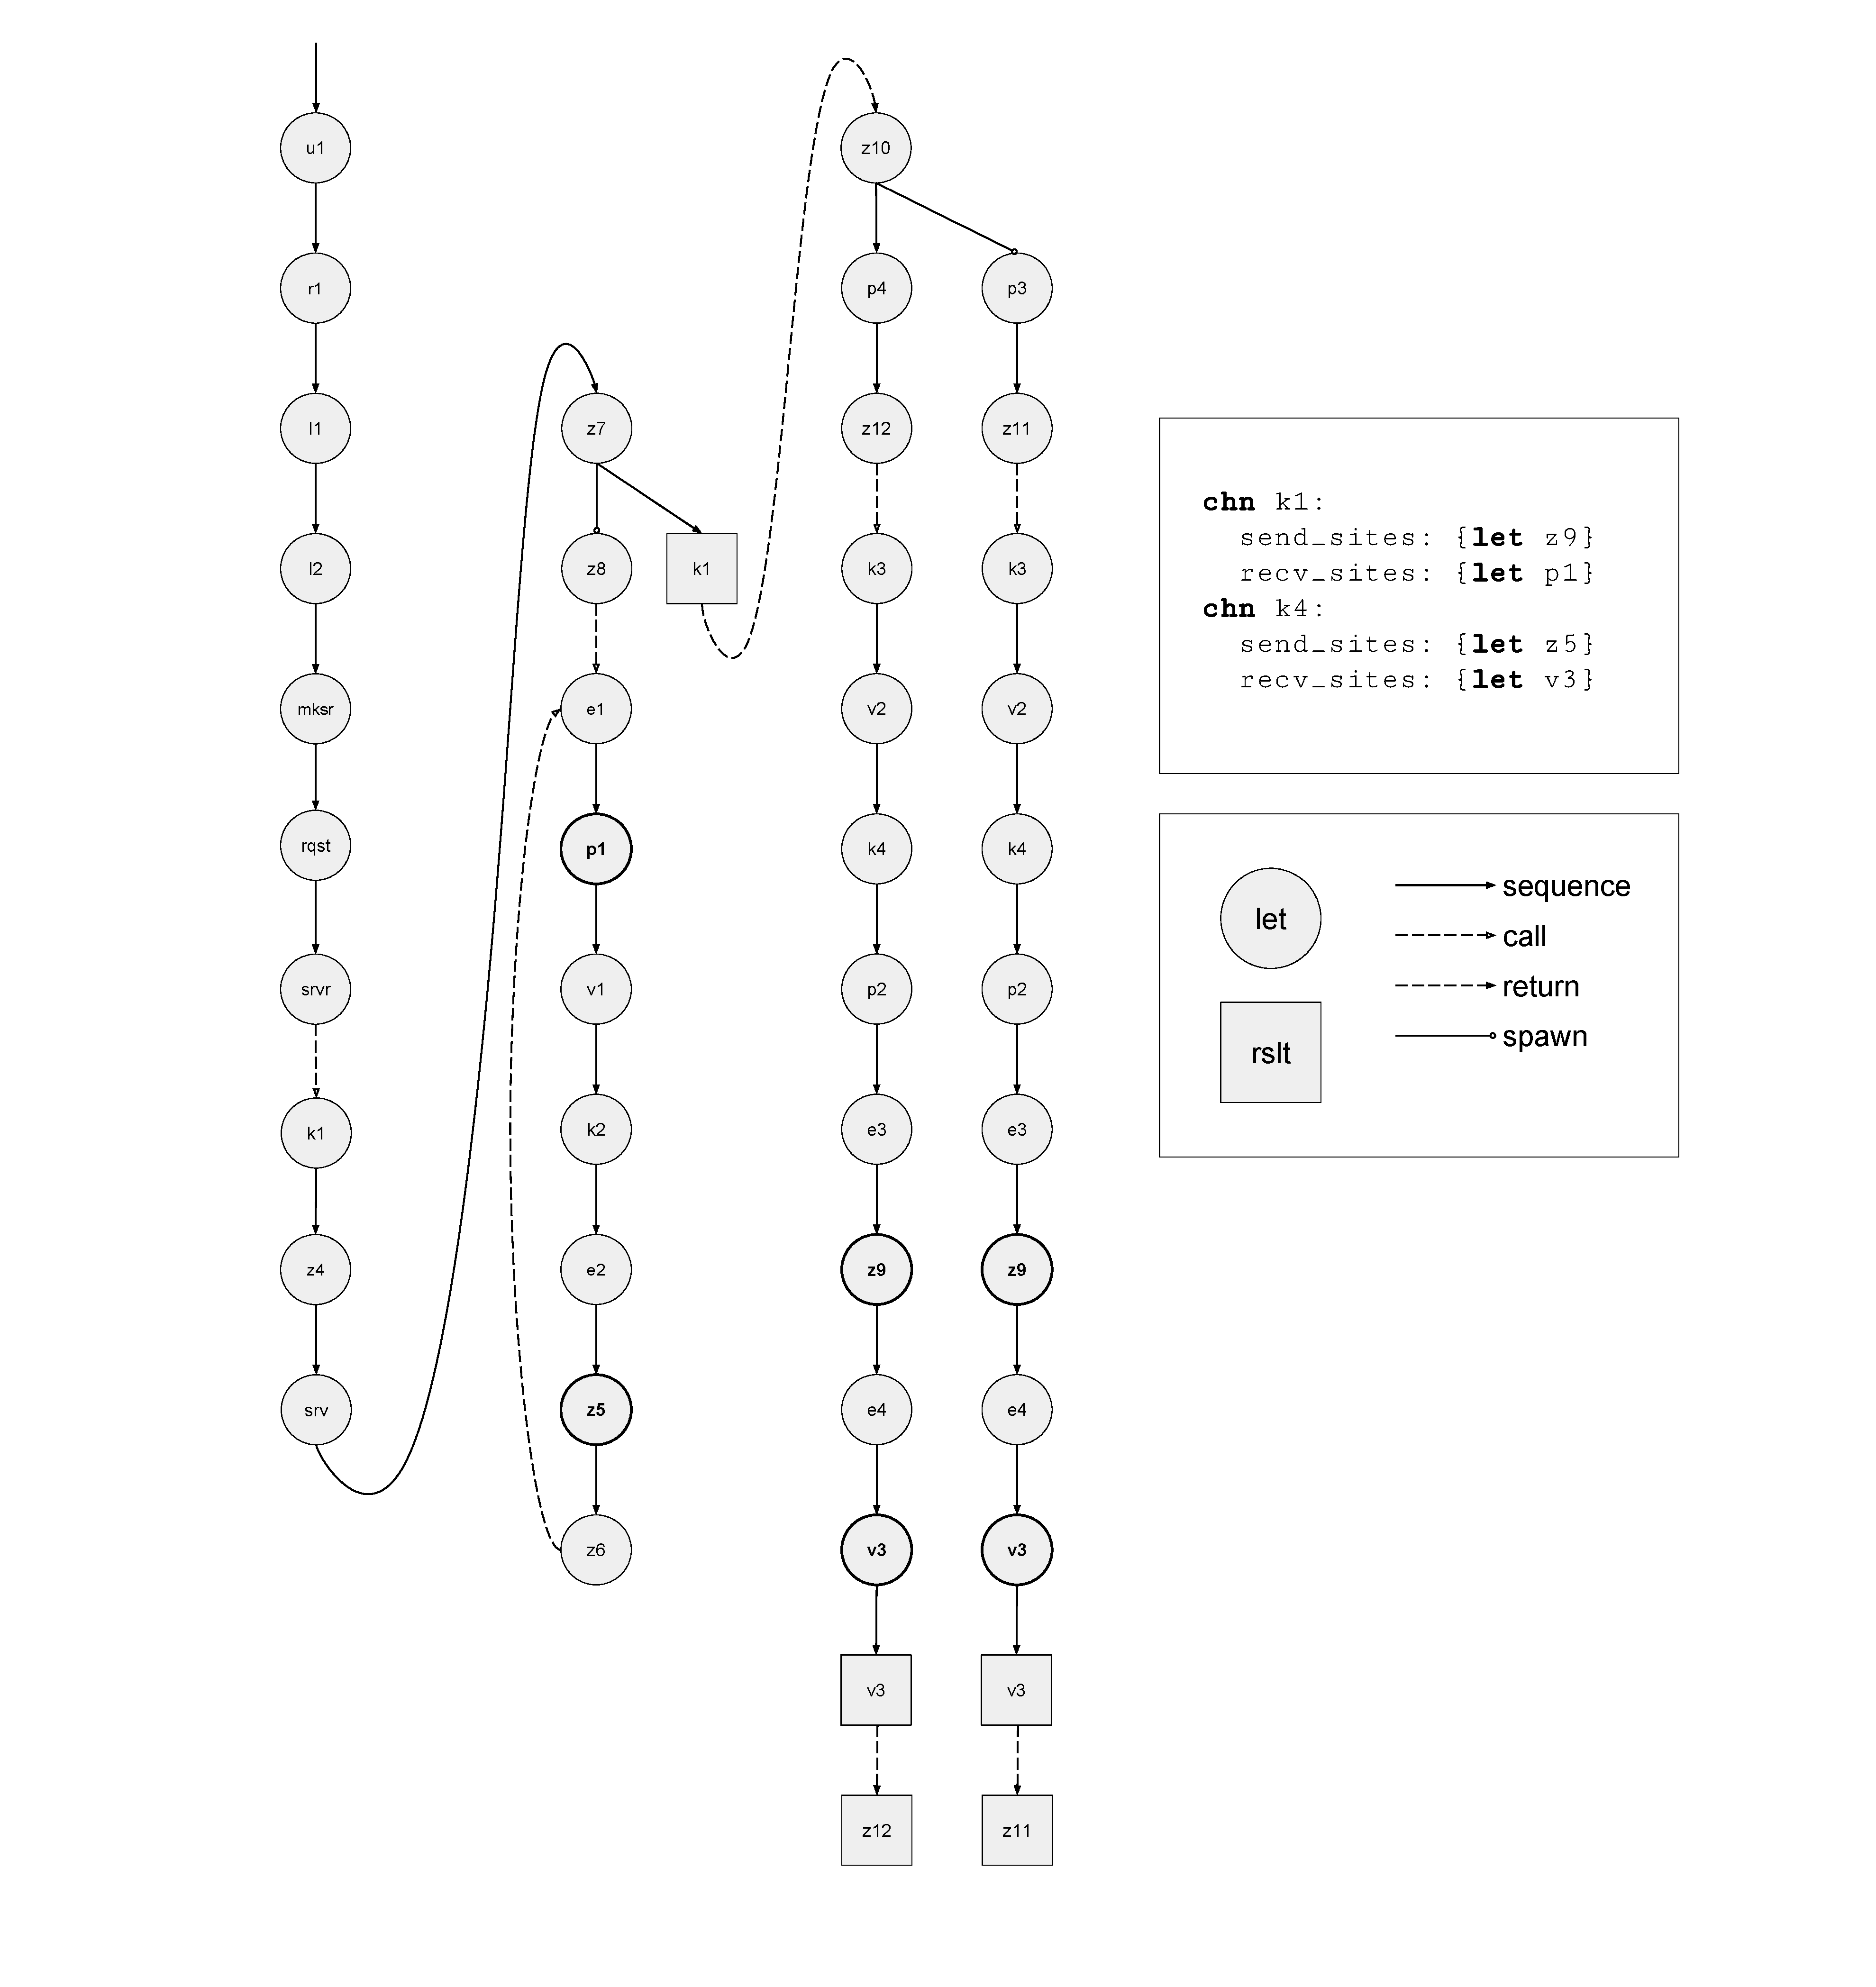
\includegraphics[scale=0.4]{cml_graph.pdf}
  
\end{document}
